% EdgeConBCE -- manuscript for Computational Biology and Chemistry.
%
% Build: pdflatex -> bibtex -> pdflatex x2, or use ../build.sh which also
% fails the build on undefined references and unresolved number macros.
%
% Every reported quantity is a macro from generated_numbers.tex, which is
% produced by pkg/make_numbers.py from the result artifacts. Do not type a
% number into this file.
\documentclass[11pt,a4paper]{article}

\usepackage[T1]{fontenc}
\usepackage[utf8]{inputenc}
\usepackage[margin=2.4cm]{geometry}
\usepackage{amsmath,amssymb}
\usepackage{graphicx}
\usepackage{booktabs}
\usepackage{siunitx}
\usepackage[round,authoryear]{natbib}
\usepackage[hidelinks]{hyperref}
\usepackage{xcolor}
\usepackage{lineno}
\usepackage{caption}

\captionsetup{font=small,labelfont=bf}
\setlength{\parskip}{0pt}
\linenumbers

\newcommand{\pending}[1]{\textcolor{red}{\textbf{[PENDING: #1]}}}
\hyphenation{turn-around re-sam-pling}
% EdgeConBCE generated manuscript numbers
% Generated by pkg/make_numbers.py -- do not edit by hand.

\newcommand{\AAdaptiveSplitAp}{0.319}
\newcommand{\AAdaptiveSplitApHi}{0.390}
\newcommand{\AAdaptiveSplitApLo}{0.246}
\newcommand{\AAdaptiveSplitApWidth}{0.145}
\newcommand{\AAdaptiveSplitAuc}{0.673}
\newcommand{\AAdaptiveSplitAucHi}{0.724}
\newcommand{\AAdaptiveSplitAucLo}{0.611}
\newcommand{\AAdaptiveSplitAucWidth}{0.113}
\newcommand{\AAdaptiveSplitCarbon}{0.160}
\newcommand{\AAdaptiveSplitCarbonHi}{0.191}
\newcommand{\AAdaptiveSplitCarbonLo}{0.132}
\newcommand{\AAdaptiveSplitCarbonWidth}{0.059}
\newcommand{\AAdaptiveSplitFOne}{0.387}
\newcommand{\AAdaptiveSplitFOneHi}{0.454}
\newcommand{\AAdaptiveSplitFOneLo}{0.307}
\newcommand{\AAdaptiveSplitFOneWidth}{0.147}
\newcommand{\AAdaptiveSplitLatency}{13.6}
\newcommand{\AAdaptiveSplitLatencyHi}{24.0}
\newcommand{\AAdaptiveSplitLatencyLo}{4.4}
\newcommand{\AAdaptiveSplitLatencyWidth}{19.6}
\newcommand{\AAdaptiveSplitMcc}{0.192}
\newcommand{\AAdaptiveSplitMccHi}{0.255}
\newcommand{\AAdaptiveSplitMccLo}{0.121}
\newcommand{\AAdaptiveSplitMccWidth}{0.134}
\newcommand{\AAdaptiveSplitRawShare}{0.285}
\newcommand{\AAdaptiveSplitRawShareHi}{0.507}
\newcommand{\AAdaptiveSplitRawShareLo}{0.087}
\newcommand{\AAdaptiveSplitRawShareWidth}{0.420}
\newcommand{\ACarbonGuardAp}{0.304}
\newcommand{\ACarbonGuardApHi}{0.379}
\newcommand{\ACarbonGuardApLo}{0.226}
\newcommand{\ACarbonGuardApWidth}{0.153}
\newcommand{\ACarbonGuardAuc}{0.658}
\newcommand{\ACarbonGuardAucHi}{0.711}
\newcommand{\ACarbonGuardAucLo}{0.595}
\newcommand{\ACarbonGuardAucWidth}{0.116}
\newcommand{\ACarbonGuardCarbon}{0.139}
\newcommand{\ACarbonGuardCarbonHi}{0.161}
\newcommand{\ACarbonGuardCarbonLo}{0.122}
\newcommand{\ACarbonGuardCarbonWidth}{0.039}
\newcommand{\ACarbonGuardFOne}{0.371}
\newcommand{\ACarbonGuardFOneHi}{0.447}
\newcommand{\ACarbonGuardFOneLo}{0.285}
\newcommand{\ACarbonGuardFOneWidth}{0.162}
\newcommand{\ACarbonGuardLatency}{6.6}
\newcommand{\ACarbonGuardLatencyHi}{14.5}
\newcommand{\ACarbonGuardLatencyLo}{1.0}
\newcommand{\ACarbonGuardLatencyWidth}{13.5}
\newcommand{\ACarbonGuardMcc}{0.165}
\newcommand{\ACarbonGuardMccHi}{0.233}
\newcommand{\ACarbonGuardMccLo}{0.091}
\newcommand{\ACarbonGuardMccWidth}{0.143}
\newcommand{\ACarbonGuardRawShare}{0.133}
\newcommand{\ACarbonGuardRawShareHi}{0.293}
\newcommand{\ACarbonGuardRawShareLo}{0.013}
\newcommand{\ACarbonGuardRawShareWidth}{0.280}
\newcommand{\ADAsVsEoAp}{-0.005}
\newcommand{\ADAsVsEoApHi}{+0.027}
\newcommand{\ADAsVsEoApLo}{-0.029}
\newcommand{\ADAsVsEoAuc}{-0.005}
\newcommand{\ADAsVsEoAucHi}{+0.021}
\newcommand{\ADAsVsEoAucLo}{-0.040}
\newcommand{\ADAsVsEoCarbon}{+0.020}
\newcommand{\ADAsVsEoCarbonHi}{+0.051}
\newcommand{\ADAsVsEoCarbonLo}{-0.007}
\newcommand{\ADAsVsEoFOne}{+0.002}
\newcommand{\ADAsVsEoFOneHi}{+0.034}
\newcommand{\ADAsVsEoFOneLo}{-0.030}
\newcommand{\ADAsVsEoLatency}{-28.8}
\newcommand{\ADAsVsEoLatencyHi}{-19.1}
\newcommand{\ADAsVsEoLatencyLo}{-37.9}
\newcommand{\ADAsVsEoMcc}{-0.017}
\newcommand{\ADAsVsEoMccHi}{+0.026}
\newcommand{\ADAsVsEoMccLo}{-0.066}
\newcommand{\ADAsVsEoRawShare}{-0.715}
\newcommand{\ADAsVsEoRawShareHi}{-0.493}
\newcommand{\ADAsVsEoRawShareLo}{-0.913}
\newcommand{\ADAsVsLoAp}{+0.015}
\newcommand{\ADAsVsLoApHi}{+0.041}
\newcommand{\ADAsVsLoApLo}{-0.001}
\newcommand{\ADAsVsLoAuc}{+0.014}
\newcommand{\ADAsVsLoAucHi}{+0.038}
\newcommand{\ADAsVsLoAucLo}{-0.004}
\newcommand{\ADAsVsLoCarbon}{+0.040}
\newcommand{\ADAsVsLoCarbonHi}{+0.071}
\newcommand{\ADAsVsLoCarbonLo}{+0.012}
\newcommand{\ADAsVsLoFOne}{+0.033}
\newcommand{\ADAsVsLoFOneHi}{+0.075}
\newcommand{\ADAsVsLoFOneLo}{+0.004}
\newcommand{\ADAsVsLoLatency}{+13.2}
\newcommand{\ADAsVsLoLatencyHi}{+23.6}
\newcommand{\ADAsVsLoLatencyLo}{+4.0}
\newcommand{\ADAsVsLoMcc}{+0.025}
\newcommand{\ADAsVsLoMccHi}{+0.065}
\newcommand{\ADAsVsLoMccLo}{-0.011}
\newcommand{\ADAsVsLoRawShare}{+0.285}
\newcommand{\ADAsVsLoRawShareHi}{+0.507}
\newcommand{\ADAsVsLoRawShareLo}{+0.087}
\newcommand{\ADCgVsAsAp}{-0.015}
\newcommand{\ADCgVsAsApHi}{-0.000}
\newcommand{\ADCgVsAsApLo}{-0.040}
\newcommand{\ADCgVsAsAuc}{-0.015}
\newcommand{\ADCgVsAsAucHi}{+0.000}
\newcommand{\ADCgVsAsAucLo}{-0.038}
\newcommand{\ADCgVsAsCarbon}{-0.021}
\newcommand{\ADCgVsAsCarbonHi}{-0.001}
\newcommand{\ADCgVsAsCarbonLo}{-0.046}
\newcommand{\ADCgVsAsFOne}{-0.016}
\newcommand{\ADCgVsAsFOneHi}{-0.001}
\newcommand{\ADCgVsAsFOneLo}{-0.039}
\newcommand{\ADCgVsAsLatency}{-7.0}
\newcommand{\ADCgVsAsLatencyHi}{+0.3}
\newcommand{\ADCgVsAsLatencyLo}{-15.8}
\newcommand{\ADCgVsAsMcc}{-0.027}
\newcommand{\ADCgVsAsMccHi}{-0.001}
\newcommand{\ADCgVsAsMccLo}{-0.064}
\newcommand{\ADCgVsAsRawShare}{-0.151}
\newcommand{\ADCgVsAsRawShareHi}{-0.007}
\newcommand{\ADCgVsAsRawShareLo}{-0.327}
\newcommand{\ADCgVsEoAp}{-0.020}
\newcommand{\ADCgVsEoApHi}{+0.017}
\newcommand{\ADCgVsEoApLo}{-0.054}
\newcommand{\ADCgVsEoAuc}{-0.020}
\newcommand{\ADCgVsEoAucHi}{+0.014}
\newcommand{\ADCgVsEoAucLo}{-0.062}
\newcommand{\ADCgVsEoCarbon}{-0.001}
\newcommand{\ADCgVsEoCarbonHi}{+0.021}
\newcommand{\ADCgVsEoCarbonLo}{-0.017}
\newcommand{\ADCgVsEoFOne}{-0.013}
\newcommand{\ADCgVsEoFOneHi}{+0.026}
\newcommand{\ADCgVsEoFOneLo}{-0.054}
\newcommand{\ADCgVsEoLatency}{-35.8}
\newcommand{\ADCgVsEoLatencyHi}{-27.8}
\newcommand{\ADCgVsEoLatencyLo}{-43.3}
\newcommand{\ADCgVsEoMcc}{-0.044}
\newcommand{\ADCgVsEoMccHi}{+0.015}
\newcommand{\ADCgVsEoMccLo}{-0.103}
\newcommand{\ADCgVsEoRawShare}{-0.867}
\newcommand{\ADCgVsEoRawShareHi}{-0.707}
\newcommand{\ADCgVsEoRawShareLo}{-0.987}
\newcommand{\ADCgVsLoAp}{+0.000}
\newcommand{\ADCgVsLoApHi}{+0.004}
\newcommand{\ADCgVsLoApLo}{-0.005}
\newcommand{\ADCgVsLoAuc}{-0.001}
\newcommand{\ADCgVsLoAucHi}{+0.003}
\newcommand{\ADCgVsLoAucLo}{-0.007}
\newcommand{\ADCgVsLoCarbon}{+0.019}
\newcommand{\ADCgVsLoCarbonHi}{+0.041}
\newcommand{\ADCgVsLoCarbonLo}{+0.002}
\newcommand{\ADCgVsLoFOne}{+0.018}
\newcommand{\ADCgVsLoFOneHi}{+0.058}
\newcommand{\ADCgVsLoFOneLo}{-0.008}
\newcommand{\ADCgVsLoLatency}{+6.2}
\newcommand{\ADCgVsLoLatencyHi}{+14.1}
\newcommand{\ADCgVsLoLatencyLo}{+0.6}
\newcommand{\ADCgVsLoMcc}{-0.002}
\newcommand{\ADCgVsLoMccHi}{+0.023}
\newcommand{\ADCgVsLoMccLo}{-0.029}
\newcommand{\ADCgVsLoRawShare}{+0.133}
\newcommand{\ADCgVsLoRawShareHi}{+0.293}
\newcommand{\ADCgVsLoRawShareLo}{+0.013}
\newcommand{\ADPasVsPeoAp}{-0.014}
\newcommand{\ADPasVsPeoApHi}{-0.005}
\newcommand{\ADPasVsPeoApLo}{-0.026}
\newcommand{\ADPasVsPeoAuc}{-0.011}
\newcommand{\ADPasVsPeoAucHi}{-0.001}
\newcommand{\ADPasVsPeoAucLo}{-0.022}
\newcommand{\ADPasVsPeoCarbon}{+0.018}
\newcommand{\ADPasVsPeoCarbonHi}{+0.046}
\newcommand{\ADPasVsPeoCarbonLo}{-0.005}
\newcommand{\ADPasVsPeoFOne}{-0.006}
\newcommand{\ADPasVsPeoFOneHi}{+0.012}
\newcommand{\ADPasVsPeoFOneLo}{-0.027}
\newcommand{\ADPasVsPeoLatency}{-21.3}
\newcommand{\ADPasVsPeoLatencyHi}{-4.1}
\newcommand{\ADPasVsPeoLatencyLo}{-37.3}
\newcommand{\ADPasVsPeoMcc}{-0.010}
\newcommand{\ADPasVsPeoMccHi}{+0.016}
\newcommand{\ADPasVsPeoMccLo}{-0.038}
\newcommand{\ADPasVsPeoRawShare}{-0.727}
\newcommand{\ADPasVsPeoRawShareHi}{-0.527}
\newcommand{\ADPasVsPeoRawShareLo}{-0.893}
\newcommand{\ADPasVsPloAp}{+0.004}
\newcommand{\ADPasVsPloApHi}{+0.010}
\newcommand{\ADPasVsPloApLo}{+0.001}
\newcommand{\ADPasVsPloAuc}{+0.002}
\newcommand{\ADPasVsPloAucHi}{+0.006}
\newcommand{\ADPasVsPloAucLo}{-0.002}
\newcommand{\ADPasVsPloCarbon}{+0.038}
\newcommand{\ADPasVsPloCarbonHi}{+0.066}
\newcommand{\ADPasVsPloCarbonLo}{+0.015}
\newcommand{\ADPasVsPloFOne}{+0.005}
\newcommand{\ADPasVsPloFOneHi}{+0.025}
\newcommand{\ADPasVsPloFOneLo}{-0.015}
\newcommand{\ADPasVsPloLatency}{+17.4}
\newcommand{\ADPasVsPloLatencyHi}{+30.1}
\newcommand{\ADPasVsPloLatencyLo}{+6.8}
\newcommand{\ADPasVsPloMcc}{+0.003}
\newcommand{\ADPasVsPloMccHi}{+0.029}
\newcommand{\ADPasVsPloMccLo}{-0.021}
\newcommand{\ADPasVsPloRawShare}{+0.273}
\newcommand{\ADPasVsPloRawShareHi}{+0.473}
\newcommand{\ADPasVsPloRawShareLo}{+0.107}
\newcommand{\AEdgeOnlyAp}{0.324}
\newcommand{\AEdgeOnlyApHi}{0.388}
\newcommand{\AEdgeOnlyApLo}{0.253}
\newcommand{\AEdgeOnlyApWidth}{0.136}
\newcommand{\AEdgeOnlyAuc}{0.678}
\newcommand{\AEdgeOnlyAucHi}{0.726}
\newcommand{\AEdgeOnlyAucLo}{0.621}
\newcommand{\AEdgeOnlyAucWidth}{0.105}
\newcommand{\AEdgeOnlyCarbon}{0.139}
\newcommand{\AEdgeOnlyCarbonHi}{0.140}
\newcommand{\AEdgeOnlyCarbonLo}{0.139}
\newcommand{\AEdgeOnlyCarbonWidth}{0.000}
\newcommand{\AEdgeOnlyFOne}{0.385}
\newcommand{\AEdgeOnlyFOneHi}{0.451}
\newcommand{\AEdgeOnlyFOneLo}{0.306}
\newcommand{\AEdgeOnlyFOneWidth}{0.145}
\newcommand{\AEdgeOnlyLatency}{42.4}
\newcommand{\AEdgeOnlyLatencyHi}{48.2}
\newcommand{\AEdgeOnlyLatencyLo}{37.2}
\newcommand{\AEdgeOnlyLatencyWidth}{11.1}
\newcommand{\AEdgeOnlyMcc}{0.209}
\newcommand{\AEdgeOnlyMccHi}{0.266}
\newcommand{\AEdgeOnlyMccLo}{0.150}
\newcommand{\AEdgeOnlyMccWidth}{0.116}
\newcommand{\AEdgeOnlyRawShare}{1.000}
\newcommand{\AEdgeOnlyRawShareHi}{1.000}
\newcommand{\AEdgeOnlyRawShareLo}{1.000}
\newcommand{\AEdgeOnlyRawShareWidth}{0.000}
\newcommand{\ALocalOnlyAp}{0.304}
\newcommand{\ALocalOnlyApHi}{0.379}
\newcommand{\ALocalOnlyApLo}{0.225}
\newcommand{\ALocalOnlyApWidth}{0.154}
\newcommand{\ALocalOnlyAuc}{0.659}
\newcommand{\ALocalOnlyAucHi}{0.712}
\newcommand{\ALocalOnlyAucLo}{0.596}
\newcommand{\ALocalOnlyAucWidth}{0.116}
\newcommand{\ALocalOnlyCarbon}{0.120}
\newcommand{\ALocalOnlyCarbonHi}{0.120}
\newcommand{\ALocalOnlyCarbonLo}{0.120}
\newcommand{\ALocalOnlyCarbonWidth}{0.000}
\newcommand{\ALocalOnlyFOne}{0.354}
\newcommand{\ALocalOnlyFOneHi}{0.426}
\newcommand{\ALocalOnlyFOneLo}{0.268}
\newcommand{\ALocalOnlyFOneWidth}{0.158}
\newcommand{\ALocalOnlyLatency}{0.4}
\newcommand{\ALocalOnlyLatencyHi}{0.5}
\newcommand{\ALocalOnlyLatencyLo}{0.4}
\newcommand{\ALocalOnlyLatencyWidth}{0.2}
\newcommand{\ALocalOnlyMcc}{0.167}
\newcommand{\ALocalOnlyMccHi}{0.229}
\newcommand{\ALocalOnlyMccLo}{0.100}
\newcommand{\ALocalOnlyMccWidth}{0.129}
\newcommand{\ALocalOnlyRawShare}{0.000}
\newcommand{\ALocalOnlyRawShareHi}{0.000}
\newcommand{\ALocalOnlyRawShareLo}{0.000}
\newcommand{\ALocalOnlyRawShareWidth}{0.000}
\newcommand{\APlmAdaptiveSplitAp}{0.298}
\newcommand{\APlmAdaptiveSplitApHi}{0.361}
\newcommand{\APlmAdaptiveSplitApLo}{0.234}
\newcommand{\APlmAdaptiveSplitApWidth}{0.127}
\newcommand{\APlmAdaptiveSplitAuc}{0.680}
\newcommand{\APlmAdaptiveSplitAucHi}{0.739}
\newcommand{\APlmAdaptiveSplitAucLo}{0.615}
\newcommand{\APlmAdaptiveSplitAucWidth}{0.124}
\newcommand{\APlmAdaptiveSplitCarbon}{0.158}
\newcommand{\APlmAdaptiveSplitCarbonHi}{0.186}
\newcommand{\APlmAdaptiveSplitCarbonLo}{0.135}
\newcommand{\APlmAdaptiveSplitCarbonWidth}{0.051}
\newcommand{\APlmAdaptiveSplitFOne}{0.386}
\newcommand{\APlmAdaptiveSplitFOneHi}{0.450}
\newcommand{\APlmAdaptiveSplitFOneLo}{0.315}
\newcommand{\APlmAdaptiveSplitFOneWidth}{0.134}
\newcommand{\APlmAdaptiveSplitLatency}{47.0}
\newcommand{\APlmAdaptiveSplitLatencyHi}{70.5}
\newcommand{\APlmAdaptiveSplitLatencyLo}{29.3}
\newcommand{\APlmAdaptiveSplitLatencyWidth}{41.2}
\newcommand{\APlmAdaptiveSplitMcc}{0.199}
\newcommand{\APlmAdaptiveSplitMccHi}{0.268}
\newcommand{\APlmAdaptiveSplitMccLo}{0.124}
\newcommand{\APlmAdaptiveSplitMccWidth}{0.144}
\newcommand{\APlmAdaptiveSplitRawShare}{0.273}
\newcommand{\APlmAdaptiveSplitRawShareHi}{0.473}
\newcommand{\APlmAdaptiveSplitRawShareLo}{0.107}
\newcommand{\APlmAdaptiveSplitRawShareWidth}{0.367}
\newcommand{\APlmConformalGuardAp}{0.298}
\newcommand{\APlmConformalGuardApHi}{0.361}
\newcommand{\APlmConformalGuardApLo}{0.234}
\newcommand{\APlmConformalGuardApWidth}{0.127}
\newcommand{\APlmConformalGuardAuc}{0.680}
\newcommand{\APlmConformalGuardAucHi}{0.739}
\newcommand{\APlmConformalGuardAucLo}{0.615}
\newcommand{\APlmConformalGuardAucWidth}{0.124}
\newcommand{\APlmConformalGuardCarbon}{0.158}
\newcommand{\APlmConformalGuardCarbonHi}{0.186}
\newcommand{\APlmConformalGuardCarbonLo}{0.135}
\newcommand{\APlmConformalGuardCarbonWidth}{0.051}
\newcommand{\APlmConformalGuardFOne}{0.386}
\newcommand{\APlmConformalGuardFOneHi}{0.450}
\newcommand{\APlmConformalGuardFOneLo}{0.315}
\newcommand{\APlmConformalGuardFOneWidth}{0.134}
\newcommand{\APlmConformalGuardLatency}{47.0}
\newcommand{\APlmConformalGuardLatencyHi}{70.5}
\newcommand{\APlmConformalGuardLatencyLo}{29.3}
\newcommand{\APlmConformalGuardLatencyWidth}{41.2}
\newcommand{\APlmConformalGuardMcc}{0.199}
\newcommand{\APlmConformalGuardMccHi}{0.268}
\newcommand{\APlmConformalGuardMccLo}{0.124}
\newcommand{\APlmConformalGuardMccWidth}{0.144}
\newcommand{\APlmConformalGuardRawShare}{0.273}
\newcommand{\APlmConformalGuardRawShareHi}{0.473}
\newcommand{\APlmConformalGuardRawShareLo}{0.107}
\newcommand{\APlmConformalGuardRawShareWidth}{0.367}
\newcommand{\APlmEdgeOnlyAp}{0.312}
\newcommand{\APlmEdgeOnlyApHi}{0.376}
\newcommand{\APlmEdgeOnlyApLo}{0.245}
\newcommand{\APlmEdgeOnlyApWidth}{0.131}
\newcommand{\APlmEdgeOnlyAuc}{0.691}
\newcommand{\APlmEdgeOnlyAucHi}{0.755}
\newcommand{\APlmEdgeOnlyAucLo}{0.623}
\newcommand{\APlmEdgeOnlyAucWidth}{0.132}
\newcommand{\APlmEdgeOnlyCarbon}{0.140}
\newcommand{\APlmEdgeOnlyCarbonHi}{0.141}
\newcommand{\APlmEdgeOnlyCarbonLo}{0.140}
\newcommand{\APlmEdgeOnlyCarbonWidth}{0.001}
\newcommand{\APlmEdgeOnlyFOne}{0.392}
\newcommand{\APlmEdgeOnlyFOneHi}{0.457}
\newcommand{\APlmEdgeOnlyFOneLo}{0.320}
\newcommand{\APlmEdgeOnlyFOneWidth}{0.137}
\newcommand{\APlmEdgeOnlyLatency}{68.3}
\newcommand{\APlmEdgeOnlyLatencyHi}{87.6}
\newcommand{\APlmEdgeOnlyLatencyLo}{54.3}
\newcommand{\APlmEdgeOnlyLatencyWidth}{33.3}
\newcommand{\APlmEdgeOnlyMcc}{0.209}
\newcommand{\APlmEdgeOnlyMccHi}{0.280}
\newcommand{\APlmEdgeOnlyMccLo}{0.133}
\newcommand{\APlmEdgeOnlyMccWidth}{0.147}
\newcommand{\APlmEdgeOnlyRawShare}{1.000}
\newcommand{\APlmEdgeOnlyRawShareHi}{1.000}
\newcommand{\APlmEdgeOnlyRawShareLo}{1.000}
\newcommand{\APlmEdgeOnlyRawShareWidth}{0.000}
\newcommand{\APlmLocalOnlyAp}{0.293}
\newcommand{\APlmLocalOnlyApHi}{0.357}
\newcommand{\APlmLocalOnlyApLo}{0.231}
\newcommand{\APlmLocalOnlyApWidth}{0.126}
\newcommand{\APlmLocalOnlyAuc}{0.678}
\newcommand{\APlmLocalOnlyAucHi}{0.739}
\newcommand{\APlmLocalOnlyAucLo}{0.614}
\newcommand{\APlmLocalOnlyAucWidth}{0.125}
\newcommand{\APlmLocalOnlyCarbon}{0.120}
\newcommand{\APlmLocalOnlyCarbonHi}{0.120}
\newcommand{\APlmLocalOnlyCarbonLo}{0.120}
\newcommand{\APlmLocalOnlyCarbonWidth}{0.000}
\newcommand{\APlmLocalOnlyFOne}{0.382}
\newcommand{\APlmLocalOnlyFOneHi}{0.446}
\newcommand{\APlmLocalOnlyFOneLo}{0.311}
\newcommand{\APlmLocalOnlyFOneWidth}{0.135}
\newcommand{\APlmLocalOnlyLatency}{29.6}
\newcommand{\APlmLocalOnlyLatencyHi}{51.0}
\newcommand{\APlmLocalOnlyLatencyLo}{17.2}
\newcommand{\APlmLocalOnlyLatencyWidth}{33.8}
\newcommand{\APlmLocalOnlyMcc}{0.195}
\newcommand{\APlmLocalOnlyMccHi}{0.259}
\newcommand{\APlmLocalOnlyMccLo}{0.124}
\newcommand{\APlmLocalOnlyMccWidth}{0.135}
\newcommand{\APlmLocalOnlyRawShare}{0.000}
\newcommand{\APlmLocalOnlyRawShareHi}{0.000}
\newcommand{\APlmLocalOnlyRawShareLo}{0.000}
\newcommand{\APlmLocalOnlyRawShareWidth}{0.000}
\newcommand{\APlmRegionEdgeAp}{0.311}
\newcommand{\APlmRegionEdgeApHi}{0.376}
\newcommand{\APlmRegionEdgeApLo}{0.241}
\newcommand{\APlmRegionEdgeApWidth}{0.135}
\newcommand{\APlmRegionEdgeAuc}{0.690}
\newcommand{\APlmRegionEdgeAucHi}{0.760}
\newcommand{\APlmRegionEdgeAucLo}{0.620}
\newcommand{\APlmRegionEdgeAucWidth}{0.139}
\newcommand{\APlmRegionEdgeCarbon}{0.140}
\newcommand{\APlmRegionEdgeCarbonHi}{0.141}
\newcommand{\APlmRegionEdgeCarbonLo}{0.140}
\newcommand{\APlmRegionEdgeCarbonWidth}{0.001}
\newcommand{\APlmRegionEdgeFOne}{0.396}
\newcommand{\APlmRegionEdgeFOneHi}{0.467}
\newcommand{\APlmRegionEdgeFOneLo}{0.310}
\newcommand{\APlmRegionEdgeFOneWidth}{0.157}
\newcommand{\APlmRegionEdgeLatency}{68.3}
\newcommand{\APlmRegionEdgeLatencyHi}{87.6}
\newcommand{\APlmRegionEdgeLatencyLo}{54.3}
\newcommand{\APlmRegionEdgeLatencyWidth}{33.3}
\newcommand{\APlmRegionEdgeMcc}{0.219}
\newcommand{\APlmRegionEdgeMccHi}{0.310}
\newcommand{\APlmRegionEdgeMccLo}{0.132}
\newcommand{\APlmRegionEdgeMccWidth}{0.178}
\newcommand{\APlmRegionEdgeRawShare}{1.000}
\newcommand{\APlmRegionEdgeRawShareHi}{1.000}
\newcommand{\APlmRegionEdgeRawShareLo}{1.000}
\newcommand{\APlmRegionEdgeRawShareWidth}{0.000}
\newcommand{\AdaptiveSplitAp}{0.315}
\newcommand{\AdaptiveSplitApHi}{0.318}
\newcommand{\AdaptiveSplitApLo}{0.311}
\newcommand{\AdaptiveSplitAuc}{0.677}
\newcommand{\AdaptiveSplitAucHi}{0.680}
\newcommand{\AdaptiveSplitAucLo}{0.673}
\newcommand{\AdaptiveSplitBytes}{62.653}
\newcommand{\AdaptiveSplitBytesHi}{73.513}
\newcommand{\AdaptiveSplitBytesLo}{46.760}
\newcommand{\AdaptiveSplitCarbon}{0.160}
\newcommand{\AdaptiveSplitCarbonHi}{0.167}
\newcommand{\AdaptiveSplitCarbonLo}{0.150}
\newcommand{\AdaptiveSplitFOne}{0.382}
\newcommand{\AdaptiveSplitFOneHi}{0.397}
\newcommand{\AdaptiveSplitFOneLo}{0.361}
\newcommand{\AdaptiveSplitLatency}{13.7}
\newcommand{\AdaptiveSplitLatencyHi}{16.1}
\newcommand{\AdaptiveSplitLatencyLo}{10.3}
\newcommand{\AdaptiveSplitMcc}{0.205}
\newcommand{\AdaptiveSplitMccHi}{0.219}
\newcommand{\AdaptiveSplitMccLo}{0.190}
\newcommand{\AdaptiveSplitRawShare}{0.287}
\newcommand{\AdaptiveSplitRawShareHi}{0.340}
\newcommand{\AdaptiveSplitRawShareLo}{0.213}
\newcommand{\AdaptiveSplitRouteRate}{0.287}
\newcommand{\AdaptiveSplitRouteRateHi}{0.340}
\newcommand{\AdaptiveSplitRouteRateLo}{0.213}
\newcommand{\AntigenBootstrapRepeats}{2000}
\newcommand{\AntigenCount}{15}
\newcommand{\BepipredAp}{0.414}
\newcommand{\BepipredAuc}{0.771}
\newcommand{\BepipredFOne}{0.460}
\newcommand{\BepipredMcc}{0.316}
\newcommand{\BepipredNumAntigens}{15}
\newcommand{\BepipredPositives}{507}
\newcommand{\BepipredResidues}{2670}
\newcommand{\BepipredThreshold}{0.1512}
\newcommand{\BiasAgreement}{0.624}
\newcommand{\BiasAtLargestN}{0.0444}
\newcommand{\BiasAtSmallestN}{0.0542}
\newcommand{\BiasCoarseGridBias}{0.0184}
\newcommand{\BiasCoarseGridPoints}{3}
\newcommand{\BiasFineGridBias}{0.0290}
\newcommand{\BiasFineGridPoints}{41}
\newcommand{\BiasGridRefN}{12}
\newcommand{\BiasLargestN}{15}
\newcommand{\BiasMetric}{MCC}
\newcommand{\BiasPositiveShareLargestN}{100}
\newcommand{\BiasReplicates}{100}
\newcommand{\BiasSmallestN}{4}
\newcommand{\BiasWorstN}{4}
\newcommand{\BiasWorstValue}{0.0542}
\newcommand{\CarbonBreakEvenPct}{13.9}
\newcommand{\CarbonBreakEvenRate}{0.139}
\newcommand{\CarbonEdgeFraction}{0.65}
\newcommand{\CarbonFlipBreakEven}{0.690}
\newcommand{\CarbonFlipEdgeFraction}{0.90}
\newcommand{\CarbonFlipLocalFraction}{0.10}
\newcommand{\CarbonFractionSettingsFlipping}{1}
\newcommand{\CarbonFractionSettingsTested}{5}
\newcommand{\CarbonGuardAp}{0.299}
\newcommand{\CarbonGuardApHi}{0.302}
\newcommand{\CarbonGuardApLo}{0.297}
\newcommand{\CarbonGuardAuc}{0.660}
\newcommand{\CarbonGuardAucHi}{0.663}
\newcommand{\CarbonGuardAucLo}{0.658}
\newcommand{\CarbonGuardBytes}{26.013}
\newcommand{\CarbonGuardBytesHi}{27.474}
\newcommand{\CarbonGuardBytesLo}{24.273}
\newcommand{\CarbonGuardCarbon}{0.139}
\newcommand{\CarbonGuardCarbonHi}{0.139}
\newcommand{\CarbonGuardCarbonLo}{0.139}
\newcommand{\CarbonGuardFOne}{0.360}
\newcommand{\CarbonGuardFOneHi}{0.378}
\newcommand{\CarbonGuardFOneLo}{0.335}
\newcommand{\CarbonGuardLatency}{6.6}
\newcommand{\CarbonGuardLatencyHi}{7.5}
\newcommand{\CarbonGuardLatencyLo}{5.8}
\newcommand{\CarbonGuardMcc}{0.173}
\newcommand{\CarbonGuardMccHi}{0.189}
\newcommand{\CarbonGuardMccLo}{0.157}
\newcommand{\CarbonGuardRawShare}{0.133}
\newcommand{\CarbonGuardRawShareHi}{0.133}
\newcommand{\CarbonGuardRawShareLo}{0.133}
\newcommand{\CarbonGuardRouteRate}{0.133}
\newcommand{\CarbonGuardRouteRateHi}{0.133}
\newcommand{\CarbonGuardRouteRateLo}{0.133}
\newcommand{\CarbonIdentityError}{0.020}
\newcommand{\CarbonLocalFraction}{0.20}
\newcommand{\CarbonPredictedAdaptive}{0.160}
\newcommand{\CarbonReconstructionError}{0e+00}
\newcommand{\CarbonSequencesChecked}{47}
\newcommand{\DAsVsEoAp}{-0.007}
\newcommand{\DAsVsEoApHi}{-0.002}
\newcommand{\DAsVsEoApLo}{-0.012}
\newcommand{\DAsVsEoAuc}{-0.005}
\newcommand{\DAsVsEoAucHi}{-0.001}
\newcommand{\DAsVsEoAucLo}{-0.010}
\newcommand{\DAsVsEoBytes}{-115.347}
\newcommand{\DAsVsEoBytesHi}{-104.487}
\newcommand{\DAsVsEoBytesLo}{-131.113}
\newcommand{\DAsVsEoCarbon}{+0.021}
\newcommand{\DAsVsEoCarbonHi}{+0.028}
\newcommand{\DAsVsEoCarbonLo}{+0.010}
\newcommand{\DAsVsEoFOne}{-0.005}
\newcommand{\DAsVsEoFOneHi}{+0.010}
\newcommand{\DAsVsEoFOneLo}{-0.024}
\newcommand{\DAsVsEoLatency}{-28.7}
\newcommand{\DAsVsEoLatencyHi}{-24.0}
\newcommand{\DAsVsEoLatencyLo}{-34.3}
\newcommand{\DAsVsEoMcc}{-0.010}
\newcommand{\DAsVsEoMccHi}{+0.004}
\newcommand{\DAsVsEoMccLo}{-0.026}
\newcommand{\DAsVsEoRawShare}{-0.713}
\newcommand{\DAsVsEoRawShareHi}{-0.660}
\newcommand{\DAsVsEoRawShareLo}{-0.787}
\newcommand{\DAsVsEoRouteRate}{\textsc{n/a}}
\newcommand{\DAsVsEoRouteRateHi}{\textsc{n/a}}
\newcommand{\DAsVsEoRouteRateLo}{\textsc{n/a}}
\newcommand{\DAsVsLoAp}{+0.016}
\newcommand{\DAsVsLoApHi}{+0.019}
\newcommand{\DAsVsLoApLo}{+0.012}
\newcommand{\DAsVsLoAuc}{+0.016}
\newcommand{\DAsVsLoAucHi}{+0.019}
\newcommand{\DAsVsLoAucLo}{+0.011}
\newcommand{\DAsVsLoBytes}{+62.653}
\newcommand{\DAsVsLoBytesHi}{+73.387}
\newcommand{\DAsVsLoBytesLo}{+46.887}
\newcommand{\DAsVsLoCarbon}{+0.040}
\newcommand{\DAsVsLoCarbonHi}{+0.047}
\newcommand{\DAsVsLoCarbonLo}{+0.031}
\newcommand{\DAsVsLoFOne}{+0.027}
\newcommand{\DAsVsLoFOneHi}{+0.034}
\newcommand{\DAsVsLoFOneLo}{+0.018}
\newcommand{\DAsVsLoLatency}{+13.3}
\newcommand{\DAsVsLoLatencyHi}{+15.6}
\newcommand{\DAsVsLoLatencyLo}{+10.0}
\newcommand{\DAsVsLoMcc}{+0.034}
\newcommand{\DAsVsLoMccHi}{+0.045}
\newcommand{\DAsVsLoMccLo}{+0.022}
\newcommand{\DAsVsLoRawShare}{+0.287}
\newcommand{\DAsVsLoRawShareHi}{+0.333}
\newcommand{\DAsVsLoRawShareLo}{+0.213}
\newcommand{\DAsVsLoRouteRate}{\textsc{n/a}}
\newcommand{\DAsVsLoRouteRateHi}{\textsc{n/a}}
\newcommand{\DAsVsLoRouteRateLo}{\textsc{n/a}}
\newcommand{\DCgVsAsAp}{-0.015}
\newcommand{\DCgVsAsApHi}{-0.011}
\newcommand{\DCgVsAsApLo}{-0.019}
\newcommand{\DCgVsAsAuc}{-0.017}
\newcommand{\DCgVsAsAucHi}{-0.011}
\newcommand{\DCgVsAsAucLo}{-0.020}
\newcommand{\DCgVsAsBytes}{-36.640}
\newcommand{\DCgVsAsBytesHi}{-19.398}
\newcommand{\DCgVsAsBytesLo}{-48.775}
\newcommand{\DCgVsAsCarbon}{-0.021}
\newcommand{\DCgVsAsCarbonHi}{-0.011}
\newcommand{\DCgVsAsCarbonLo}{-0.029}
\newcommand{\DCgVsAsFOne}{-0.022}
\newcommand{\DCgVsAsFOneHi}{-0.014}
\newcommand{\DCgVsAsFOneLo}{-0.030}
\newcommand{\DCgVsAsLatency}{-7.1}
\newcommand{\DCgVsAsLatencyHi}{-3.4}
\newcommand{\DCgVsAsLatencyLo}{-9.5}
\newcommand{\DCgVsAsMcc}{-0.033}
\newcommand{\DCgVsAsMccHi}{-0.022}
\newcommand{\DCgVsAsMccLo}{-0.046}
\newcommand{\DCgVsAsRawShare}{-0.153}
\newcommand{\DCgVsAsRawShareHi}{-0.080}
\newcommand{\DCgVsAsRawShareLo}{-0.207}
\newcommand{\DCgVsAsRouteRate}{-0.153}
\newcommand{\DCgVsAsRouteRateHi}{-0.080}
\newcommand{\DCgVsAsRouteRateLo}{-0.207}
\newcommand{\DCgVsEoAp}{-0.022}
\newcommand{\DCgVsEoApHi}{-0.018}
\newcommand{\DCgVsEoApLo}{-0.027}
\newcommand{\DCgVsEoAuc}{-0.022}
\newcommand{\DCgVsEoAucHi}{-0.019}
\newcommand{\DCgVsEoAucLo}{-0.024}
\newcommand{\DCgVsEoBytes}{-151.987}
\newcommand{\DCgVsEoBytesHi}{-150.500}
\newcommand{\DCgVsEoBytesLo}{-153.727}
\newcommand{\DCgVsEoCarbon}{-0.001}
\newcommand{\DCgVsEoCarbonHi}{-0.001}
\newcommand{\DCgVsEoCarbonLo}{-0.001}
\newcommand{\DCgVsEoFOne}{-0.027}
\newcommand{\DCgVsEoFOneHi}{-0.008}
\newcommand{\DCgVsEoFOneLo}{-0.048}
\newcommand{\DCgVsEoLatency}{-35.8}
\newcommand{\DCgVsEoLatencyHi}{-32.7}
\newcommand{\DCgVsEoLatencyLo}{-39.1}
\newcommand{\DCgVsEoMcc}{-0.042}
\newcommand{\DCgVsEoMccHi}{-0.025}
\newcommand{\DCgVsEoMccLo}{-0.059}
\newcommand{\DCgVsEoRawShare}{-0.867}
\newcommand{\DCgVsEoRawShareHi}{-0.867}
\newcommand{\DCgVsEoRawShareLo}{-0.867}
\newcommand{\DCgVsEoRouteRate}{\textsc{n/a}}
\newcommand{\DCgVsEoRouteRateHi}{\textsc{n/a}}
\newcommand{\DCgVsEoRouteRateLo}{\textsc{n/a}}
\newcommand{\DCgVsLoAp}{+0.000}
\newcommand{\DCgVsLoApHi}{+0.003}
\newcommand{\DCgVsLoApLo}{-0.002}
\newcommand{\DCgVsLoAuc}{-0.001}
\newcommand{\DCgVsLoAucHi}{+0.001}
\newcommand{\DCgVsLoAucLo}{-0.003}
\newcommand{\DCgVsLoBytes}{+26.013}
\newcommand{\DCgVsLoBytesHi}{+27.613}
\newcommand{\DCgVsLoBytesLo}{+24.273}
\newcommand{\DCgVsLoCarbon}{+0.019}
\newcommand{\DCgVsLoCarbonHi}{+0.019}
\newcommand{\DCgVsLoCarbonLo}{+0.019}
\newcommand{\DCgVsLoFOne}{+0.005}
\newcommand{\DCgVsLoFOneHi}{+0.010}
\newcommand{\DCgVsLoFOneLo}{+0.000}
\newcommand{\DCgVsLoLatency}{+6.2}
\newcommand{\DCgVsLoLatencyHi}{+7.0}
\newcommand{\DCgVsLoLatencyLo}{+5.4}
\newcommand{\DCgVsLoMcc}{+0.001}
\newcommand{\DCgVsLoMccHi}{+0.011}
\newcommand{\DCgVsLoMccLo}{-0.008}
\newcommand{\DCgVsLoRawShare}{+0.133}
\newcommand{\DCgVsLoRawShareHi}{+0.133}
\newcommand{\DCgVsLoRawShareLo}{+0.133}
\newcommand{\DCgVsLoRouteRate}{\textsc{n/a}}
\newcommand{\DCgVsLoRouteRateHi}{\textsc{n/a}}
\newcommand{\DCgVsLoRouteRateLo}{\textsc{n/a}}
\newcommand{\DPasVsPeoAp}{-0.015}
\newcommand{\DPasVsPeoApHi}{-0.008}
\newcommand{\DPasVsPeoApLo}{-0.021}
\newcommand{\DPasVsPeoAuc}{-0.012}
\newcommand{\DPasVsPeoAucHi}{-0.006}
\newcommand{\DPasVsPeoAucLo}{-0.018}
\newcommand{\DPasVsPeoBytes}{-129.727}
\newcommand{\DPasVsPeoBytesHi}{-107.071}
\newcommand{\DPasVsPeoBytesLo}{-150.321}
\newcommand{\DPasVsPeoCarbon}{+0.018}
\newcommand{\DPasVsPeoCarbonHi}{+0.038}
\newcommand{\DPasVsPeoCarbonLo}{+0.002}
\newcommand{\DPasVsPeoFOne}{-0.005}
\newcommand{\DPasVsPeoFOneHi}{+0.003}
\newcommand{\DPasVsPeoFOneLo}{-0.014}
\newcommand{\DPasVsPeoLatency}{-21.3}
\newcommand{\DPasVsPeoLatencyHi}{-11.0}
\newcommand{\DPasVsPeoLatencyLo}{-33.5}
\newcommand{\DPasVsPeoMcc}{-0.008}
\newcommand{\DPasVsPeoMccHi}{+0.005}
\newcommand{\DPasVsPeoMccLo}{-0.021}
\newcommand{\DPasVsPeoRawShare}{-0.727}
\newcommand{\DPasVsPeoRawShareHi}{-0.593}
\newcommand{\DPasVsPeoRawShareLo}{-0.847}
\newcommand{\DPasVsPeoRouteRate}{\textsc{n/a}}
\newcommand{\DPasVsPeoRouteRateHi}{\textsc{n/a}}
\newcommand{\DPasVsPeoRouteRateLo}{\textsc{n/a}}
\newcommand{\DPasVsPloAp}{+0.004}
\newcommand{\DPasVsPloApHi}{+0.006}
\newcommand{\DPasVsPloApLo}{+0.002}
\newcommand{\DPasVsPloAuc}{+0.002}
\newcommand{\DPasVsPloAucHi}{+0.004}
\newcommand{\DPasVsPloAucLo}{-0.001}
\newcommand{\DPasVsPloBytes}{+48.273}
\newcommand{\DPasVsPloBytesHi}{+71.242}
\newcommand{\DPasVsPloBytesLo}{+27.772}
\newcommand{\DPasVsPloCarbon}{+0.038}
\newcommand{\DPasVsPloCarbonHi}{+0.057}
\newcommand{\DPasVsPloCarbonLo}{+0.022}
\newcommand{\DPasVsPloFOne}{+0.006}
\newcommand{\DPasVsPloFOneHi}{+0.014}
\newcommand{\DPasVsPloFOneLo}{-0.001}
\newcommand{\DPasVsPloLatency}{+17.4}
\newcommand{\DPasVsPloLatencyHi}{+25.5}
\newcommand{\DPasVsPloLatencyLo}{+10.3}
\newcommand{\DPasVsPloMcc}{+0.006}
\newcommand{\DPasVsPloMccHi}{+0.016}
\newcommand{\DPasVsPloMccLo}{-0.002}
\newcommand{\DPasVsPloRawShare}{+0.273}
\newcommand{\DPasVsPloRawShareHi}{+0.413}
\newcommand{\DPasVsPloRawShareLo}{+0.153}
\newcommand{\DPasVsPloRouteRate}{\textsc{n/a}}
\newcommand{\DPasVsPloRouteRateHi}{\textsc{n/a}}
\newcommand{\DPasVsPloRouteRateLo}{\textsc{n/a}}
\newcommand{\DPeoVsEoAp}{-0.013}
\newcommand{\DPeoVsEoApHi}{-0.005}
\newcommand{\DPeoVsEoApLo}{-0.020}
\newcommand{\DPeoVsEoAuc}{+0.013}
\newcommand{\DPeoVsEoAucHi}{+0.023}
\newcommand{\DPeoVsEoAucLo}{+0.003}
\newcommand{\DPeoVsEoBytes}{+0.000}
\newcommand{\DPeoVsEoBytesHi}{+0.000}
\newcommand{\DPeoVsEoBytesLo}{+0.000}
\newcommand{\DPeoVsEoCarbon}{+0.001}
\newcommand{\DPeoVsEoCarbonHi}{+0.001}
\newcommand{\DPeoVsEoCarbonLo}{+0.000}
\newcommand{\DPeoVsEoFOne}{+0.006}
\newcommand{\DPeoVsEoFOneHi}{+0.016}
\newcommand{\DPeoVsEoFOneLo}{-0.004}
\newcommand{\DPeoVsEoLatency}{+25.9}
\newcommand{\DPeoVsEoLatencyHi}{+41.3}
\newcommand{\DPeoVsEoLatencyLo}{+14.9}
\newcommand{\DPeoVsEoMcc}{-0.001}
\newcommand{\DPeoVsEoMccHi}{+0.011}
\newcommand{\DPeoVsEoMccLo}{-0.011}
\newcommand{\DPeoVsEoRawShare}{+0.000}
\newcommand{\DPeoVsEoRawShareHi}{+0.000}
\newcommand{\DPeoVsEoRawShareLo}{+0.000}
\newcommand{\DPeoVsEoRouteRate}{\textsc{n/a}}
\newcommand{\DPeoVsEoRouteRateHi}{\textsc{n/a}}
\newcommand{\DPeoVsEoRouteRateLo}{\textsc{n/a}}
\newcommand{\DPloVsLoAp}{-0.009}
\newcommand{\DPloVsLoApHi}{-0.000}
\newcommand{\DPloVsLoApLo}{-0.018}
\newcommand{\DPloVsLoAuc}{+0.020}
\newcommand{\DPloVsLoAucHi}{+0.032}
\newcommand{\DPloVsLoAucLo}{+0.010}
\newcommand{\DPloVsLoBytes}{+0.000}
\newcommand{\DPloVsLoBytesHi}{+0.000}
\newcommand{\DPloVsLoBytesLo}{+0.000}
\newcommand{\DPloVsLoCarbon}{+0.000}
\newcommand{\DPloVsLoCarbonHi}{+0.000}
\newcommand{\DPloVsLoCarbonLo}{+0.000}
\newcommand{\DPloVsLoFOne}{+0.027}
\newcommand{\DPloVsLoFOneHi}{+0.061}
\newcommand{\DPloVsLoFOneLo}{+0.004}
\newcommand{\DPloVsLoLatency}{+29.2}
\newcommand{\DPloVsLoLatencyHi}{+36.0}
\newcommand{\DPloVsLoLatencyLo}{+23.3}
\newcommand{\DPloVsLoMcc}{+0.029}
\newcommand{\DPloVsLoMccHi}{+0.045}
\newcommand{\DPloVsLoMccLo}{+0.013}
\newcommand{\DPloVsLoRawShare}{+0.000}
\newcommand{\DPloVsLoRawShareHi}{+0.000}
\newcommand{\DPloVsLoRawShareLo}{+0.000}
\newcommand{\DPloVsLoRouteRate}{\textsc{n/a}}
\newcommand{\DPloVsLoRouteRateHi}{\textsc{n/a}}
\newcommand{\DPloVsLoRouteRateLo}{\textsc{n/a}}
\newcommand{\DPreVsPeoAp}{-0.001}
\newcommand{\DPreVsPeoApHi}{+0.001}
\newcommand{\DPreVsPeoApLo}{-0.003}
\newcommand{\DPreVsPeoAuc}{-0.000}
\newcommand{\DPreVsPeoAucHi}{+0.003}
\newcommand{\DPreVsPeoAucLo}{-0.003}
\newcommand{\DPreVsPeoBytes}{+0.000}
\newcommand{\DPreVsPeoBytesHi}{+0.000}
\newcommand{\DPreVsPeoBytesLo}{+0.000}
\newcommand{\DPreVsPeoCarbon}{+0.000}
\newcommand{\DPreVsPeoCarbonHi}{+0.000}
\newcommand{\DPreVsPeoCarbonLo}{+0.000}
\newcommand{\DPreVsPeoFOne}{+0.004}
\newcommand{\DPreVsPeoFOneHi}{+0.013}
\newcommand{\DPreVsPeoFOneLo}{-0.006}
\newcommand{\DPreVsPeoLatency}{+0.0}
\newcommand{\DPreVsPeoLatencyHi}{+0.0}
\newcommand{\DPreVsPeoLatencyLo}{+0.0}
\newcommand{\DPreVsPeoMcc}{+0.010}
\newcommand{\DPreVsPeoMccHi}{+0.022}
\newcommand{\DPreVsPeoMccLo}{-0.001}
\newcommand{\DPreVsPeoRawShare}{+0.000}
\newcommand{\DPreVsPeoRawShareHi}{+0.000}
\newcommand{\DPreVsPeoRawShareLo}{+0.000}
\newcommand{\DPreVsPeoRouteRate}{\textsc{n/a}}
\newcommand{\DPreVsPeoRouteRateHi}{\textsc{n/a}}
\newcommand{\DPreVsPeoRouteRateLo}{\textsc{n/a}}
\newcommand{\DPreVsPloAp}{+0.017}
\newcommand{\DPreVsPloApHi}{+0.024}
\newcommand{\DPreVsPloApLo}{+0.012}
\newcommand{\DPreVsPloAuc}{+0.013}
\newcommand{\DPreVsPloAucHi}{+0.020}
\newcommand{\DPreVsPloAucLo}{+0.006}
\newcommand{\DPreVsPloBytes}{+178.000}
\newcommand{\DPreVsPloBytesHi}{+178.000}
\newcommand{\DPreVsPloBytesLo}{+178.000}
\newcommand{\DPreVsPloCarbon}{+0.020}
\newcommand{\DPreVsPloCarbonHi}{+0.020}
\newcommand{\DPreVsPloCarbonLo}{+0.020}
\newcommand{\DPreVsPloFOne}{+0.015}
\newcommand{\DPreVsPloFOneHi}{+0.031}
\newcommand{\DPreVsPloFOneLo}{-0.001}
\newcommand{\DPreVsPloLatency}{+38.8}
\newcommand{\DPreVsPloLatencyHi}{+50.7}
\newcommand{\DPreVsPloLatencyLo}{+30.8}
\newcommand{\DPreVsPloMcc}{+0.024}
\newcommand{\DPreVsPloMccHi}{+0.045}
\newcommand{\DPreVsPloMccLo}{+0.002}
\newcommand{\DPreVsPloRawShare}{+1.000}
\newcommand{\DPreVsPloRawShareHi}{+1.000}
\newcommand{\DPreVsPloRawShareLo}{+1.000}
\newcommand{\DPreVsPloRouteRate}{\textsc{n/a}}
\newcommand{\DPreVsPloRouteRateHi}{\textsc{n/a}}
\newcommand{\DPreVsPloRouteRateLo}{\textsc{n/a}}
\newcommand{\EdgeOnlyAp}{0.322}
\newcommand{\EdgeOnlyApHi}{0.326}
\newcommand{\EdgeOnlyApLo}{0.317}
\newcommand{\EdgeOnlyAuc}{0.682}
\newcommand{\EdgeOnlyAucHi}{0.685}
\newcommand{\EdgeOnlyAucLo}{0.680}
\newcommand{\EdgeOnlyBytes}{178.000}
\newcommand{\EdgeOnlyBytesHi}{178.000}
\newcommand{\EdgeOnlyBytesLo}{178.000}
\newcommand{\EdgeOnlyCarbon}{0.139}
\newcommand{\EdgeOnlyCarbonHi}{0.139}
\newcommand{\EdgeOnlyCarbonLo}{0.139}
\newcommand{\EdgeOnlyFOne}{0.387}
\newcommand{\EdgeOnlyFOneHi}{0.394}
\newcommand{\EdgeOnlyFOneLo}{0.380}
\newcommand{\EdgeOnlyLatency}{42.4}
\newcommand{\EdgeOnlyLatencyHi}{46.3}
\newcommand{\EdgeOnlyLatencyLo}{38.7}
\newcommand{\EdgeOnlyMcc}{0.215}
\newcommand{\EdgeOnlyMccHi}{0.221}
\newcommand{\EdgeOnlyMccLo}{0.208}
\newcommand{\EdgeOnlyRawShare}{1.000}
\newcommand{\EdgeOnlyRawShareHi}{1.000}
\newcommand{\EdgeOnlyRawShareLo}{1.000}
\newcommand{\EdgeOnlyRouteRate}{\textsc{n/a}}
\newcommand{\EdgeOnlyRouteRateHi}{\textsc{n/a}}
\newcommand{\EdgeOnlyRouteRateLo}{\textsc{n/a}}
\newcommand{\EmbodiedDeclaredEdge}{0.2125}
\newcommand{\EmbodiedDeclaredLocal}{0.6000}
\newcommand{\EmbodiedEffectiveEdge}{0.1381}
\newcommand{\EmbodiedEffectiveLocal}{0.1200}
\newcommand{\EmbodiedImpliedEdge}{0.1381}
\newcommand{\EmbodiedImpliedLocal}{0.1200}
\newcommand{\IedbAdaptiveSplitAp}{0.249}
\newcommand{\IedbAdaptiveSplitAuc}{0.640}
\newcommand{\IedbAdaptiveSplitFOne}{0.318}
\newcommand{\IedbAdaptiveSplitMcc}{0.167}
\newcommand{\IedbBpThreeCompared}{358}
\newcommand{\IedbCarbonGuardAp}{0.245}
\newcommand{\IedbCarbonGuardAuc}{0.645}
\newcommand{\IedbCarbonGuardFOne}{0.317}
\newcommand{\IedbCarbonGuardMcc}{0.155}
\newcommand{\IedbEdgeOnlyAp}{0.230}
\newcommand{\IedbEdgeOnlyAuc}{0.637}
\newcommand{\IedbEdgeOnlyFOne}{0.275}
\newcommand{\IedbEdgeOnlyMcc}{0.154}
\newcommand{\IedbExactOverlap}{0}
\newcommand{\IedbIdOverlap}{0}
\newcommand{\IedbKmerSize}{10}
\newcommand{\IedbLengthMax}{595}
\newcommand{\IedbLengthMin}{45}
\newcommand{\IedbLocalOnlyAp}{0.247}
\newcommand{\IedbLocalOnlyAuc}{0.645}
\newcommand{\IedbLocalOnlyFOne}{0.321}
\newcommand{\IedbLocalOnlyMcc}{0.161}
\newcommand{\IedbMaxContainment}{0.000}
\newcommand{\IedbNumPolicies}{9}
\newcommand{\IedbPlmAdaptiveSplitAp}{0.187}
\newcommand{\IedbPlmAdaptiveSplitAuc}{0.575}
\newcommand{\IedbPlmAdaptiveSplitFOne}{0.209}
\newcommand{\IedbPlmAdaptiveSplitMcc}{0.066}
\newcommand{\IedbPlmConformalGuardAp}{0.187}
\newcommand{\IedbPlmConformalGuardAuc}{0.575}
\newcommand{\IedbPlmConformalGuardFOne}{0.209}
\newcommand{\IedbPlmConformalGuardMcc}{0.066}
\newcommand{\IedbPlmEdgeOnlyAp}{0.185}
\newcommand{\IedbPlmEdgeOnlyAuc}{0.576}
\newcommand{\IedbPlmEdgeOnlyFOne}{0.205}
\newcommand{\IedbPlmEdgeOnlyMcc}{0.068}
\newcommand{\IedbPlmLocalOnlyAp}{0.191}
\newcommand{\IedbPlmLocalOnlyAuc}{0.585}
\newcommand{\IedbPlmLocalOnlyFOne}{0.211}
\newcommand{\IedbPlmLocalOnlyMcc}{0.067}
\newcommand{\IedbPlmRegionEdgeAp}{0.186}
\newcommand{\IedbPlmRegionEdgeAuc}{0.577}
\newcommand{\IedbPlmRegionEdgeFOne}{0.185}
\newcommand{\IedbPlmRegionEdgeMcc}{0.064}
\newcommand{\IedbSourceFile}{IEDBSeqsNotSharedAt20ID.fasta}
\newcommand{\IedbSourceSequences}{3560}
\newcommand{\IedbSubsetTest}{47}
\newcommand{\IedbSubsetTrain}{205}
\newcommand{\LocalOnlyAp}{0.299}
\newcommand{\LocalOnlyApHi}{0.299}
\newcommand{\LocalOnlyApLo}{0.299}
\newcommand{\LocalOnlyAuc}{0.661}
\newcommand{\LocalOnlyAucHi}{0.661}
\newcommand{\LocalOnlyAucLo}{0.661}
\newcommand{\LocalOnlyBytes}{0.000}
\newcommand{\LocalOnlyBytesHi}{0.000}
\newcommand{\LocalOnlyBytesLo}{0.000}
\newcommand{\LocalOnlyCarbon}{0.120}
\newcommand{\LocalOnlyCarbonHi}{0.120}
\newcommand{\LocalOnlyCarbonLo}{0.120}
\newcommand{\LocalOnlyFOne}{0.355}
\newcommand{\LocalOnlyFOneHi}{0.373}
\newcommand{\LocalOnlyFOneLo}{0.328}
\newcommand{\LocalOnlyLatency}{0.4}
\newcommand{\LocalOnlyLatencyHi}{0.5}
\newcommand{\LocalOnlyLatencyLo}{0.4}
\newcommand{\LocalOnlyMcc}{0.171}
\newcommand{\LocalOnlyMccHi}{0.178}
\newcommand{\LocalOnlyMccLo}{0.164}
\newcommand{\LocalOnlyRawShare}{0.000}
\newcommand{\LocalOnlyRawShareHi}{0.000}
\newcommand{\LocalOnlyRawShareLo}{0.000}
\newcommand{\LocalOnlyRouteRate}{\textsc{n/a}}
\newcommand{\LocalOnlyRouteRateHi}{\textsc{n/a}}
\newcommand{\LocalOnlyRouteRateLo}{\textsc{n/a}}
\newcommand{\NestedBpThreeDeltaAp}{-0.0036}
\newcommand{\NestedBpThreeDeltaApHi}{+0.0041}
\newcommand{\NestedBpThreeDeltaApLo}{-0.0135}
\newcommand{\NestedBpThreeDeltaAuc}{-0.0005}
\newcommand{\NestedBpThreeDeltaAucHi}{+0.0021}
\newcommand{\NestedBpThreeDeltaAucLo}{-0.0033}
\newcommand{\NestedBpThreeDeltaFOne}{-0.0095}
\newcommand{\NestedBpThreeDeltaFOneHi}{+0.0094}
\newcommand{\NestedBpThreeDeltaFOneLo}{-0.0343}
\newcommand{\NestedBpThreeDeltaMcc}{-0.0329}
\newcommand{\NestedBpThreeDeltaMccHi}{+0.0088}
\newcommand{\NestedBpThreeDeltaMccLo}{-0.0955}
\newcommand{\NestedBpThreeFusionAp}{0.4149}
\newcommand{\NestedBpThreeFusionAuc}{0.7701}
\newcommand{\NestedBpThreeFusionFOne}{0.4630}
\newcommand{\NestedBpThreeFusionMcc}{0.3227}
\newcommand{\NestedBpThreeLossesAp}{5}
\newcommand{\NestedBpThreeLossesAuc}{7}
\newcommand{\NestedBpThreeLossesFOne}{8}
\newcommand{\NestedBpThreeLossesMcc}{8}
\newcommand{\NestedBpThreeMdeAp}{0.0132}
\newcommand{\NestedBpThreeMdeAuc}{0.0040}
\newcommand{\NestedBpThreeMdeFOne}{0.0331}
\newcommand{\NestedBpThreeMdeMcc}{0.0822}
\newcommand{\NestedBpThreePAp}{0.925}
\newcommand{\NestedBpThreePAuc}{0.925}
\newcommand{\NestedBpThreePFOne}{0.762}
\newcommand{\NestedBpThreePMcc}{0.561}
\newcommand{\NestedBpThreePSignAp}{0.424}
\newcommand{\NestedBpThreePSignAuc}{1.000}
\newcommand{\NestedBpThreePSignFOne}{1.000}
\newcommand{\NestedBpThreePSignMcc}{1.000}
\newcommand{\NestedBpThreePooledDeltaAp}{+0.0023}
\newcommand{\NestedBpThreePooledDeltaAuc}{-0.0025}
\newcommand{\NestedBpThreePooledDeltaFOne}{-0.0009}
\newcommand{\NestedBpThreePooledDeltaMcc}{-0.0015}
\newcommand{\NestedBpThreePositives}{507}
\newcommand{\NestedBpThreeReferenceAp}{0.4126}
\newcommand{\NestedBpThreeReferenceAuc}{0.7726}
\newcommand{\NestedBpThreeReferenceFOne}{0.4639}
\newcommand{\NestedBpThreeReferenceMcc}{0.3242}
\newcommand{\NestedBpThreeResidues}{2670}
\newcommand{\NestedBpThreeSdAp}{0.0183}
\newcommand{\NestedBpThreeSdAuc}{0.0055}
\newcommand{\NestedBpThreeSdFOne}{0.0458}
\newcommand{\NestedBpThreeSdMcc}{0.1137}
\newcommand{\NestedBpThreeSequences}{15}
\newcommand{\NestedBpThreeTiesAp}{1}
\newcommand{\NestedBpThreeTiesAuc}{1}
\newcommand{\NestedBpThreeTiesFOne}{0}
\newcommand{\NestedBpThreeTiesMcc}{0}
\newcommand{\NestedBpThreeWeightMax}{0.90}
\newcommand{\NestedBpThreeWeightMedian}{0.90}
\newcommand{\NestedBpThreeWeightMin}{0.55}
\newcommand{\NestedBpThreeWinsAp}{9}
\newcommand{\NestedBpThreeWinsAuc}{7}
\newcommand{\NestedBpThreeWinsFOne}{7}
\newcommand{\NestedBpThreeWinsMcc}{7}
\newcommand{\NestedIedbDeltaAp}{-0.0029}
\newcommand{\NestedIedbDeltaApHi}{+0.0042}
\newcommand{\NestedIedbDeltaApLo}{-0.0128}
\newcommand{\NestedIedbDeltaAuc}{+0.0008}
\newcommand{\NestedIedbDeltaAucHi}{+0.0027}
\newcommand{\NestedIedbDeltaAucLo}{-0.0010}
\newcommand{\NestedIedbDeltaFOne}{-0.0010}
\newcommand{\NestedIedbDeltaFOneHi}{+0.0014}
\newcommand{\NestedIedbDeltaFOneLo}{-0.0036}
\newcommand{\NestedIedbDeltaMcc}{+0.0014}
\newcommand{\NestedIedbDeltaMccHi}{+0.0066}
\newcommand{\NestedIedbDeltaMccLo}{-0.0037}
\newcommand{\NestedIedbFusionAp}{0.2485}
\newcommand{\NestedIedbFusionAuc}{0.6456}
\newcommand{\NestedIedbFusionFOne}{0.3210}
\newcommand{\NestedIedbFusionMcc}{0.1606}
\newcommand{\NestedIedbLossesAp}{21}
\newcommand{\NestedIedbLossesAuc}{22}
\newcommand{\NestedIedbLossesFOne}{17}
\newcommand{\NestedIedbLossesMcc}{15}
\newcommand{\NestedIedbMdeAp}{0.0125}
\newcommand{\NestedIedbMdeAuc}{0.0027}
\newcommand{\NestedIedbMdeFOne}{0.0036}
\newcommand{\NestedIedbMdeMcc}{0.0073}
\newcommand{\NestedIedbPAp}{0.156}
\newcommand{\NestedIedbPAuc}{0.485}
\newcommand{\NestedIedbPFOne}{0.925}
\newcommand{\NestedIedbPMcc}{0.418}
\newcommand{\NestedIedbPSignAp}{0.560}
\newcommand{\NestedIedbPSignAuc}{0.771}
\newcommand{\NestedIedbPSignFOne}{0.627}
\newcommand{\NestedIedbPSignMcc}{0.200}
\newcommand{\NestedIedbPooledDeltaAp}{+0.0022}
\newcommand{\NestedIedbPooledDeltaAuc}{+0.0004}
\newcommand{\NestedIedbPooledDeltaFOne}{-0.0015}
\newcommand{\NestedIedbPooledDeltaMcc}{-0.0024}
\newcommand{\NestedIedbPositives}{2169}
\newcommand{\NestedIedbReferenceAp}{0.2463}
\newcommand{\NestedIedbReferenceAuc}{0.6452}
\newcommand{\NestedIedbReferenceFOne}{0.3225}
\newcommand{\NestedIedbReferenceMcc}{0.1629}
\newcommand{\NestedIedbResidues}{14408}
\newcommand{\NestedIedbSdAp}{0.0307}
\newcommand{\NestedIedbSdAuc}{0.0066}
\newcommand{\NestedIedbSdFOne}{0.0087}
\newcommand{\NestedIedbSdMcc}{0.0179}
\newcommand{\NestedIedbSequences}{47}
\newcommand{\NestedIedbTiesAp}{0}
\newcommand{\NestedIedbTiesAuc}{0}
\newcommand{\NestedIedbTiesFOne}{9}
\newcommand{\NestedIedbTiesMcc}{8}
\newcommand{\NestedIedbWeightMax}{0.95}
\newcommand{\NestedIedbWeightMedian}{0.95}
\newcommand{\NestedIedbWeightMin}{0.85}
\newcommand{\NestedIedbWinsAp}{26}
\newcommand{\NestedIedbWinsAuc}{25}
\newcommand{\NestedIedbWinsFOne}{21}
\newcommand{\NestedIedbWinsMcc}{24}
\newcommand{\NumSeeds}{10}
\newcommand{\OperationalEdge}{2.4e-03}
\newcommand{\OperationalLocal}{7.0e-06}
\newcommand{\PlmAdaptiveSplitAp}{0.294}
\newcommand{\PlmAdaptiveSplitApHi}{0.303}
\newcommand{\PlmAdaptiveSplitApLo}{0.284}
\newcommand{\PlmAdaptiveSplitAuc}{0.683}
\newcommand{\PlmAdaptiveSplitAucHi}{0.694}
\newcommand{\PlmAdaptiveSplitAucLo}{0.672}
\newcommand{\PlmAdaptiveSplitBytes}{48.273}
\newcommand{\PlmAdaptiveSplitBytesHi}{71.007}
\newcommand{\PlmAdaptiveSplitBytesLo}{28.266}
\newcommand{\PlmAdaptiveSplitCarbon}{0.158}
\newcommand{\PlmAdaptiveSplitCarbonHi}{0.177}
\newcommand{\PlmAdaptiveSplitCarbonLo}{0.142}
\newcommand{\PlmAdaptiveSplitFOne}{0.388}
\newcommand{\PlmAdaptiveSplitFOneHi}{0.396}
\newcommand{\PlmAdaptiveSplitFOneLo}{0.380}
\newcommand{\PlmAdaptiveSplitLatency}{47.0}
\newcommand{\PlmAdaptiveSplitLatencyHi}{58.3}
\newcommand{\PlmAdaptiveSplitLatencyLo}{36.2}
\newcommand{\PlmAdaptiveSplitMcc}{0.206}
\newcommand{\PlmAdaptiveSplitMccHi}{0.218}
\newcommand{\PlmAdaptiveSplitMccLo}{0.193}
\newcommand{\PlmAdaptiveSplitRawShare}{0.273}
\newcommand{\PlmAdaptiveSplitRawShareHi}{0.413}
\newcommand{\PlmAdaptiveSplitRawShareLo}{0.160}
\newcommand{\PlmAdaptiveSplitRouteRate}{0.273}
\newcommand{\PlmAdaptiveSplitRouteRateHi}{0.407}
\newcommand{\PlmAdaptiveSplitRouteRateLo}{0.147}
\newcommand{\PlmConformalGuardAp}{0.294}
\newcommand{\PlmConformalGuardApHi}{0.303}
\newcommand{\PlmConformalGuardApLo}{0.285}
\newcommand{\PlmConformalGuardAuc}{0.683}
\newcommand{\PlmConformalGuardAucHi}{0.695}
\newcommand{\PlmConformalGuardAucLo}{0.673}
\newcommand{\PlmConformalGuardBytes}{48.273}
\newcommand{\PlmConformalGuardBytesHi}{71.022}
\newcommand{\PlmConformalGuardBytesLo}{28.079}
\newcommand{\PlmConformalGuardCarbon}{0.158}
\newcommand{\PlmConformalGuardCarbonHi}{0.177}
\newcommand{\PlmConformalGuardCarbonLo}{0.142}
\newcommand{\PlmConformalGuardFOne}{0.388}
\newcommand{\PlmConformalGuardFOneHi}{0.396}
\newcommand{\PlmConformalGuardFOneLo}{0.380}
\newcommand{\PlmConformalGuardLatency}{47.0}
\newcommand{\PlmConformalGuardLatencyHi}{58.5}
\newcommand{\PlmConformalGuardLatencyLo}{35.5}
\newcommand{\PlmConformalGuardMcc}{0.206}
\newcommand{\PlmConformalGuardMccHi}{0.219}
\newcommand{\PlmConformalGuardMccLo}{0.193}
\newcommand{\PlmConformalGuardRawShare}{0.273}
\newcommand{\PlmConformalGuardRawShareHi}{0.413}
\newcommand{\PlmConformalGuardRawShareLo}{0.160}
\newcommand{\PlmConformalGuardRouteRate}{0.273}
\newcommand{\PlmConformalGuardRouteRateHi}{0.413}
\newcommand{\PlmConformalGuardRouteRateLo}{0.160}
\newcommand{\PlmEdgeOnlyAp}{0.309}
\newcommand{\PlmEdgeOnlyApHi}{0.315}
\newcommand{\PlmEdgeOnlyApLo}{0.303}
\newcommand{\PlmEdgeOnlyAuc}{0.695}
\newcommand{\PlmEdgeOnlyAucHi}{0.704}
\newcommand{\PlmEdgeOnlyAucLo}{0.687}
\newcommand{\PlmEdgeOnlyBytes}{178.000}
\newcommand{\PlmEdgeOnlyBytesHi}{178.000}
\newcommand{\PlmEdgeOnlyBytesLo}{178.000}
\newcommand{\PlmEdgeOnlyCarbon}{0.140}
\newcommand{\PlmEdgeOnlyCarbonHi}{0.141}
\newcommand{\PlmEdgeOnlyCarbonLo}{0.140}
\newcommand{\PlmEdgeOnlyFOne}{0.393}
\newcommand{\PlmEdgeOnlyFOneHi}{0.397}
\newcommand{\PlmEdgeOnlyFOneLo}{0.389}
\newcommand{\PlmEdgeOnlyLatency}{68.4}
\newcommand{\PlmEdgeOnlyLatencyHi}{84.5}
\newcommand{\PlmEdgeOnlyLatencyLo}{56.7}
\newcommand{\PlmEdgeOnlyMcc}{0.214}
\newcommand{\PlmEdgeOnlyMccHi}{0.221}
\newcommand{\PlmEdgeOnlyMccLo}{0.208}
\newcommand{\PlmEdgeOnlyRawShare}{1.000}
\newcommand{\PlmEdgeOnlyRawShareHi}{1.000}
\newcommand{\PlmEdgeOnlyRawShareLo}{1.000}
\newcommand{\PlmEdgeOnlyRouteRate}{\textsc{n/a}}
\newcommand{\PlmEdgeOnlyRouteRateHi}{\textsc{n/a}}
\newcommand{\PlmEdgeOnlyRouteRateLo}{\textsc{n/a}}
\newcommand{\PlmLocalOnlyAp}{0.290}
\newcommand{\PlmLocalOnlyApHi}{0.299}
\newcommand{\PlmLocalOnlyApLo}{0.281}
\newcommand{\PlmLocalOnlyAuc}{0.682}
\newcommand{\PlmLocalOnlyAucHi}{0.693}
\newcommand{\PlmLocalOnlyAucLo}{0.671}
\newcommand{\PlmLocalOnlyBytes}{0.000}
\newcommand{\PlmLocalOnlyBytesHi}{0.000}
\newcommand{\PlmLocalOnlyBytesLo}{0.000}
\newcommand{\PlmLocalOnlyCarbon}{0.120}
\newcommand{\PlmLocalOnlyCarbonHi}{0.120}
\newcommand{\PlmLocalOnlyCarbonLo}{0.120}
\newcommand{\PlmLocalOnlyFOne}{0.382}
\newcommand{\PlmLocalOnlyFOneHi}{0.394}
\newcommand{\PlmLocalOnlyFOneLo}{0.371}
\newcommand{\PlmLocalOnlyLatency}{29.6}
\newcommand{\PlmLocalOnlyLatencyHi}{36.4}
\newcommand{\PlmLocalOnlyLatencyLo}{23.6}
\newcommand{\PlmLocalOnlyMcc}{0.200}
\newcommand{\PlmLocalOnlyMccHi}{0.217}
\newcommand{\PlmLocalOnlyMccLo}{0.185}
\newcommand{\PlmLocalOnlyRawShare}{0.000}
\newcommand{\PlmLocalOnlyRawShareHi}{0.000}
\newcommand{\PlmLocalOnlyRawShareLo}{0.000}
\newcommand{\PlmLocalOnlyRouteRate}{\textsc{n/a}}
\newcommand{\PlmLocalOnlyRouteRateHi}{\textsc{n/a}}
\newcommand{\PlmLocalOnlyRouteRateLo}{\textsc{n/a}}
\newcommand{\PlmRegionEdgeAp}{0.308}
\newcommand{\PlmRegionEdgeApHi}{0.313}
\newcommand{\PlmRegionEdgeApLo}{0.302}
\newcommand{\PlmRegionEdgeAuc}{0.694}
\newcommand{\PlmRegionEdgeAucHi}{0.702}
\newcommand{\PlmRegionEdgeAucLo}{0.687}
\newcommand{\PlmRegionEdgeBytes}{178.000}
\newcommand{\PlmRegionEdgeBytesHi}{178.000}
\newcommand{\PlmRegionEdgeBytesLo}{178.000}
\newcommand{\PlmRegionEdgeCarbon}{0.140}
\newcommand{\PlmRegionEdgeCarbonHi}{0.141}
\newcommand{\PlmRegionEdgeCarbonLo}{0.140}
\newcommand{\PlmRegionEdgeFOne}{0.397}
\newcommand{\PlmRegionEdgeFOneHi}{0.407}
\newcommand{\PlmRegionEdgeFOneLo}{0.387}
\newcommand{\PlmRegionEdgeLatency}{68.4}
\newcommand{\PlmRegionEdgeLatencyHi}{85.0}
\newcommand{\PlmRegionEdgeLatencyLo}{56.9}
\newcommand{\PlmRegionEdgeMcc}{0.225}
\newcommand{\PlmRegionEdgeMccHi}{0.237}
\newcommand{\PlmRegionEdgeMccLo}{0.212}
\newcommand{\PlmRegionEdgeRawShare}{1.000}
\newcommand{\PlmRegionEdgeRawShareHi}{1.000}
\newcommand{\PlmRegionEdgeRawShareLo}{1.000}
\newcommand{\PlmRegionEdgeRouteRate}{\textsc{n/a}}
\newcommand{\PlmRegionEdgeRouteRateHi}{\textsc{n/a}}
\newcommand{\PlmRegionEdgeRouteRateLo}{\textsc{n/a}}
\newcommand{\PolicyPairsComputed}{36}
\newcommand{\ProvenanceEmbodiedCarbon}{amortized estimate from device metadata}
\newcommand{\ProvenanceEnergy}{estimated from fixed power and latency}
\newcommand{\ProvenanceLatency}{timed benchmark execution}
\newcommand{\ProvenanceOperationalCarbon}{estimated from energy and grid intensity}
\newcommand{\QualityIntervalsComputed}{144}
\newcommand{\RouteBudgetMax}{0.50}
\newcommand{\SAsVsEoApLosses}{8}
\newcommand{\SAsVsEoApP}{0.1094}
\newcommand{\SAsVsEoApWins}{2}
\newcommand{\SAsVsEoAucLosses}{7}
\newcommand{\SAsVsEoAucP}{0.3438}
\newcommand{\SAsVsEoAucWins}{3}
\newcommand{\SAsVsEoBytesLosses}{0}
\newcommand{\SAsVsEoBytesP}{0.0020}
\newcommand{\SAsVsEoBytesWins}{10}
\newcommand{\SAsVsEoCarbonLosses}{9}
\newcommand{\SAsVsEoCarbonP}{0.0215}
\newcommand{\SAsVsEoCarbonWins}{1}
\newcommand{\SAsVsEoFOneLosses}{3}
\newcommand{\SAsVsEoFOneP}{0.3438}
\newcommand{\SAsVsEoFOneWins}{7}
\newcommand{\SAsVsEoLatencyLosses}{0}
\newcommand{\SAsVsEoLatencyP}{0.0020}
\newcommand{\SAsVsEoLatencyWins}{10}
\newcommand{\SAsVsEoMccLosses}{4}
\newcommand{\SAsVsEoMccP}{0.7539}
\newcommand{\SAsVsEoMccWins}{6}
\newcommand{\SAsVsEoRawShareLosses}{0}
\newcommand{\SAsVsEoRawShareP}{0.0020}
\newcommand{\SAsVsEoRawShareWins}{10}
\newcommand{\SAsVsLoApLosses}{0}
\newcommand{\SAsVsLoApP}{0.0039}
\newcommand{\SAsVsLoApWins}{9}
\newcommand{\SAsVsLoAucLosses}{0}
\newcommand{\SAsVsLoAucP}{0.0039}
\newcommand{\SAsVsLoAucWins}{9}
\newcommand{\SAsVsLoBytesLosses}{9}
\newcommand{\SAsVsLoBytesP}{0.0039}
\newcommand{\SAsVsLoBytesWins}{0}
\newcommand{\SAsVsLoCarbonLosses}{9}
\newcommand{\SAsVsLoCarbonP}{0.0039}
\newcommand{\SAsVsLoCarbonWins}{0}
\newcommand{\SAsVsLoFOneLosses}{0}
\newcommand{\SAsVsLoFOneP}{0.0039}
\newcommand{\SAsVsLoFOneWins}{9}
\newcommand{\SAsVsLoLatencyLosses}{9}
\newcommand{\SAsVsLoLatencyP}{0.0039}
\newcommand{\SAsVsLoLatencyWins}{0}
\newcommand{\SAsVsLoMccLosses}{0}
\newcommand{\SAsVsLoMccP}{0.0039}
\newcommand{\SAsVsLoMccWins}{9}
\newcommand{\SAsVsLoRawShareLosses}{9}
\newcommand{\SAsVsLoRawShareP}{0.0039}
\newcommand{\SAsVsLoRawShareWins}{0}
\newcommand{\SCgVsAsApLosses}{9}
\newcommand{\SCgVsAsApP}{0.0215}
\newcommand{\SCgVsAsApWins}{1}
\newcommand{\SCgVsAsAucLosses}{9}
\newcommand{\SCgVsAsAucP}{0.0215}
\newcommand{\SCgVsAsAucWins}{1}
\newcommand{\SCgVsAsBytesLosses}{1}
\newcommand{\SCgVsAsBytesP}{0.0215}
\newcommand{\SCgVsAsBytesWins}{9}
\newcommand{\SCgVsAsCarbonLosses}{1}
\newcommand{\SCgVsAsCarbonP}{0.0215}
\newcommand{\SCgVsAsCarbonWins}{9}
\newcommand{\SCgVsAsFOneLosses}{10}
\newcommand{\SCgVsAsFOneP}{0.0020}
\newcommand{\SCgVsAsFOneWins}{0}
\newcommand{\SCgVsAsLatencyLosses}{1}
\newcommand{\SCgVsAsLatencyP}{0.0215}
\newcommand{\SCgVsAsLatencyWins}{9}
\newcommand{\SCgVsAsMccLosses}{10}
\newcommand{\SCgVsAsMccP}{0.0020}
\newcommand{\SCgVsAsMccWins}{0}
\newcommand{\SCgVsAsRawShareLosses}{1}
\newcommand{\SCgVsAsRawShareP}{0.0215}
\newcommand{\SCgVsAsRawShareWins}{9}
\newcommand{\SCgVsEoApLosses}{10}
\newcommand{\SCgVsEoApP}{0.0020}
\newcommand{\SCgVsEoApWins}{0}
\newcommand{\SCgVsEoAucLosses}{10}
\newcommand{\SCgVsEoAucP}{0.0020}
\newcommand{\SCgVsEoAucWins}{0}
\newcommand{\SCgVsEoBytesLosses}{0}
\newcommand{\SCgVsEoBytesP}{0.0020}
\newcommand{\SCgVsEoBytesWins}{10}
\newcommand{\SCgVsEoCarbonLosses}{0}
\newcommand{\SCgVsEoCarbonP}{0.0020}
\newcommand{\SCgVsEoCarbonWins}{10}
\newcommand{\SCgVsEoFOneLosses}{7}
\newcommand{\SCgVsEoFOneP}{0.3438}
\newcommand{\SCgVsEoFOneWins}{3}
\newcommand{\SCgVsEoLatencyLosses}{0}
\newcommand{\SCgVsEoLatencyP}{0.0020}
\newcommand{\SCgVsEoLatencyWins}{10}
\newcommand{\SCgVsEoMccLosses}{10}
\newcommand{\SCgVsEoMccP}{0.0020}
\newcommand{\SCgVsEoMccWins}{0}
\newcommand{\SCgVsEoRawShareLosses}{0}
\newcommand{\SCgVsEoRawShareP}{0.0020}
\newcommand{\SCgVsEoRawShareWins}{10}
\newcommand{\SCgVsLoApLosses}{5}
\newcommand{\SCgVsLoApP}{1.0000}
\newcommand{\SCgVsLoApWins}{5}
\newcommand{\SCgVsLoAucLosses}{7}
\newcommand{\SCgVsLoAucP}{0.3438}
\newcommand{\SCgVsLoAucWins}{3}
\newcommand{\SCgVsLoBytesLosses}{10}
\newcommand{\SCgVsLoBytesP}{0.0020}
\newcommand{\SCgVsLoBytesWins}{0}
\newcommand{\SCgVsLoCarbonLosses}{10}
\newcommand{\SCgVsLoCarbonP}{0.0020}
\newcommand{\SCgVsLoCarbonWins}{0}
\newcommand{\SCgVsLoFOneLosses}{3}
\newcommand{\SCgVsLoFOneP}{0.3438}
\newcommand{\SCgVsLoFOneWins}{7}
\newcommand{\SCgVsLoLatencyLosses}{10}
\newcommand{\SCgVsLoLatencyP}{0.0020}
\newcommand{\SCgVsLoLatencyWins}{0}
\newcommand{\SCgVsLoMccLosses}{5}
\newcommand{\SCgVsLoMccP}{1.0000}
\newcommand{\SCgVsLoMccWins}{5}
\newcommand{\SCgVsLoRawShareLosses}{10}
\newcommand{\SCgVsLoRawShareP}{0.0020}
\newcommand{\SCgVsLoRawShareWins}{0}
\newcommand{\SPasVsPeoApLosses}{9}
\newcommand{\SPasVsPeoApP}{0.0215}
\newcommand{\SPasVsPeoApWins}{1}
\newcommand{\SPasVsPeoAucLosses}{9}
\newcommand{\SPasVsPeoAucP}{0.0215}
\newcommand{\SPasVsPeoAucWins}{1}
\newcommand{\SPasVsPeoBytesLosses}{0}
\newcommand{\SPasVsPeoBytesP}{0.0020}
\newcommand{\SPasVsPeoBytesWins}{10}
\newcommand{\SPasVsPeoCarbonLosses}{7}
\newcommand{\SPasVsPeoCarbonP}{0.3438}
\newcommand{\SPasVsPeoCarbonWins}{3}
\newcommand{\SPasVsPeoFOneLosses}{6}
\newcommand{\SPasVsPeoFOneP}{0.7539}
\newcommand{\SPasVsPeoFOneWins}{4}
\newcommand{\SPasVsPeoLatencyLosses}{1}
\newcommand{\SPasVsPeoLatencyP}{0.0215}
\newcommand{\SPasVsPeoLatencyWins}{9}
\newcommand{\SPasVsPeoMccLosses}{7}
\newcommand{\SPasVsPeoMccP}{0.3438}
\newcommand{\SPasVsPeoMccWins}{3}
\newcommand{\SPasVsPeoRawShareLosses}{0}
\newcommand{\SPasVsPeoRawShareP}{0.0020}
\newcommand{\SPasVsPeoRawShareWins}{10}
\newcommand{\SPasVsPloApLosses}{0}
\newcommand{\SPasVsPloApP}{0.0039}
\newcommand{\SPasVsPloApWins}{9}
\newcommand{\SPasVsPloAucLosses}{4}
\newcommand{\SPasVsPloAucP}{1.0000}
\newcommand{\SPasVsPloAucWins}{5}
\newcommand{\SPasVsPloBytesLosses}{9}
\newcommand{\SPasVsPloBytesP}{0.0039}
\newcommand{\SPasVsPloBytesWins}{0}
\newcommand{\SPasVsPloCarbonLosses}{9}
\newcommand{\SPasVsPloCarbonP}{0.0039}
\newcommand{\SPasVsPloCarbonWins}{0}
\newcommand{\SPasVsPloFOneLosses}{2}
\newcommand{\SPasVsPloFOneP}{0.1797}
\newcommand{\SPasVsPloFOneWins}{7}
\newcommand{\SPasVsPloLatencyLosses}{9}
\newcommand{\SPasVsPloLatencyP}{0.0039}
\newcommand{\SPasVsPloLatencyWins}{0}
\newcommand{\SPasVsPloMccLosses}{3}
\newcommand{\SPasVsPloMccP}{0.5078}
\newcommand{\SPasVsPloMccWins}{6}
\newcommand{\SPasVsPloRawShareLosses}{9}
\newcommand{\SPasVsPloRawShareP}{0.0039}
\newcommand{\SPasVsPloRawShareWins}{0}
\newcommand{\SPeoVsEoApLosses}{8}
\newcommand{\SPeoVsEoApP}{0.1094}
\newcommand{\SPeoVsEoApWins}{2}
\newcommand{\SPeoVsEoAucLosses}{3}
\newcommand{\SPeoVsEoAucP}{0.3438}
\newcommand{\SPeoVsEoAucWins}{7}
\newcommand{\SPeoVsEoBytesLosses}{0}
\newcommand{\SPeoVsEoBytesP}{1.0000}
\newcommand{\SPeoVsEoBytesWins}{0}
\newcommand{\SPeoVsEoCarbonLosses}{10}
\newcommand{\SPeoVsEoCarbonP}{0.0020}
\newcommand{\SPeoVsEoCarbonWins}{0}
\newcommand{\SPeoVsEoFOneLosses}{4}
\newcommand{\SPeoVsEoFOneP}{0.7539}
\newcommand{\SPeoVsEoFOneWins}{6}
\newcommand{\SPeoVsEoLatencyLosses}{10}
\newcommand{\SPeoVsEoLatencyP}{0.0020}
\newcommand{\SPeoVsEoLatencyWins}{0}
\newcommand{\SPeoVsEoMccLosses}{6}
\newcommand{\SPeoVsEoMccP}{0.7539}
\newcommand{\SPeoVsEoMccWins}{4}
\newcommand{\SPeoVsEoRawShareLosses}{0}
\newcommand{\SPeoVsEoRawShareP}{1.0000}
\newcommand{\SPeoVsEoRawShareWins}{0}
\newcommand{\SPloVsLoApLosses}{7}
\newcommand{\SPloVsLoApP}{0.3438}
\newcommand{\SPloVsLoApWins}{3}
\newcommand{\SPloVsLoAucLosses}{1}
\newcommand{\SPloVsLoAucP}{0.0215}
\newcommand{\SPloVsLoAucWins}{9}
\newcommand{\SPloVsLoBytesLosses}{0}
\newcommand{\SPloVsLoBytesP}{1.0000}
\newcommand{\SPloVsLoBytesWins}{0}
\newcommand{\SPloVsLoCarbonLosses}{10}
\newcommand{\SPloVsLoCarbonP}{0.0020}
\newcommand{\SPloVsLoCarbonWins}{0}
\newcommand{\SPloVsLoFOneLosses}{3}
\newcommand{\SPloVsLoFOneP}{0.3438}
\newcommand{\SPloVsLoFOneWins}{7}
\newcommand{\SPloVsLoLatencyLosses}{10}
\newcommand{\SPloVsLoLatencyP}{0.0020}
\newcommand{\SPloVsLoLatencyWins}{0}
\newcommand{\SPloVsLoMccLosses}{2}
\newcommand{\SPloVsLoMccP}{0.1094}
\newcommand{\SPloVsLoMccWins}{8}
\newcommand{\SPloVsLoRawShareLosses}{0}
\newcommand{\SPloVsLoRawShareP}{1.0000}
\newcommand{\SPloVsLoRawShareWins}{0}
\newcommand{\SPreVsPeoApLosses}{7}
\newcommand{\SPreVsPeoApP}{0.3438}
\newcommand{\SPreVsPeoApWins}{3}
\newcommand{\SPreVsPeoAucLosses}{5}
\newcommand{\SPreVsPeoAucP}{1.0000}
\newcommand{\SPreVsPeoAucWins}{5}
\newcommand{\SPreVsPeoBytesLosses}{0}
\newcommand{\SPreVsPeoBytesP}{1.0000}
\newcommand{\SPreVsPeoBytesWins}{0}
\newcommand{\SPreVsPeoCarbonLosses}{0}
\newcommand{\SPreVsPeoCarbonP}{1.0000}
\newcommand{\SPreVsPeoCarbonWins}{0}
\newcommand{\SPreVsPeoFOneLosses}{3}
\newcommand{\SPreVsPeoFOneP}{0.3438}
\newcommand{\SPreVsPeoFOneWins}{7}
\newcommand{\SPreVsPeoLatencyLosses}{0}
\newcommand{\SPreVsPeoLatencyP}{1.0000}
\newcommand{\SPreVsPeoLatencyWins}{0}
\newcommand{\SPreVsPeoMccLosses}{2}
\newcommand{\SPreVsPeoMccP}{0.1094}
\newcommand{\SPreVsPeoMccWins}{8}
\newcommand{\SPreVsPeoRawShareLosses}{0}
\newcommand{\SPreVsPeoRawShareP}{1.0000}
\newcommand{\SPreVsPeoRawShareWins}{0}
\newcommand{\SPreVsPloApLosses}{0}
\newcommand{\SPreVsPloApP}{0.0020}
\newcommand{\SPreVsPloApWins}{10}
\newcommand{\SPreVsPloAucLosses}{1}
\newcommand{\SPreVsPloAucP}{0.0215}
\newcommand{\SPreVsPloAucWins}{9}
\newcommand{\SPreVsPloBytesLosses}{10}
\newcommand{\SPreVsPloBytesP}{0.0020}
\newcommand{\SPreVsPloBytesWins}{0}
\newcommand{\SPreVsPloCarbonLosses}{10}
\newcommand{\SPreVsPloCarbonP}{0.0020}
\newcommand{\SPreVsPloCarbonWins}{0}
\newcommand{\SPreVsPloFOneLosses}{3}
\newcommand{\SPreVsPloFOneP}{0.3438}
\newcommand{\SPreVsPloFOneWins}{7}
\newcommand{\SPreVsPloLatencyLosses}{10}
\newcommand{\SPreVsPloLatencyP}{0.0020}
\newcommand{\SPreVsPloLatencyWins}{0}
\newcommand{\SPreVsPloMccLosses}{3}
\newcommand{\SPreVsPloMccP}{0.3438}
\newcommand{\SPreVsPloMccWins}{7}
\newcommand{\SPreVsPloRawShareLosses}{10}
\newcommand{\SPreVsPloRawShareP}{0.0020}
\newcommand{\SPreVsPloRawShareWins}{0}
\newcommand{\ScaleBreakEvenMeasured}{0.139}
\newcommand{\ScaleCrossoverFactor}{13.0}
\newcommand{\ScaleCrossoverParams}{104}
\newcommand{\ScaleFirstCleanBreakEven}{0.341}
\newcommand{\ScaleFirstCleanCheckpoint}{esm2\_t30\_150M\_UR50D}
\newcommand{\ScaleLargeBreakEven}{0.639}
\newcommand{\ScaleLargeEdgeCost}{0.3325}
\newcommand{\ScaleLargeFactor}{81}
\newcommand{\ScaleMidBreakEven}{0.341}
\newcommand{\ScaleMidEdgeCost}{0.1821}
\newcommand{\ScaleMidFactor}{19}
\newcommand{\ScaleOperationalShareEdge}{1.7}
\newcommand{\ScaleSmallBreakEven}{0.186}
\newcommand{\ScaleSmallEdgeCost}{0.1475}
\newcommand{\ScaleSmallFactor}{4}
\newcommand{\ScaleVerdictInverts}{yes}
\newcommand{\SeedFirst}{42}
\newcommand{\SeedLast}{51}
\newcommand{\SurveyAssessed}{12}
\newcommand{\SurveyClean}{6}
\newcommand{\SurveyLeakage}{3}
\newcommand{\SurveyLeakageShare}{33}
\newcommand{\SurveyStatingBasis}{9}
\newcommand{\SurveyUnreported}{3}
\newcommand{\ThresholdGridSize}{91}
\newcommand{\TunedBpThreeDeltaAp}{+0.0043}
\newcommand{\TunedBpThreeDeltaAuc}{+0.0018}
\newcommand{\TunedBpThreeDeltaFOne}{+0.0071}
\newcommand{\TunedBpThreeDeltaMcc}{+0.0115}
\newcommand{\TunedBpThreeFusionAp}{0.419}
\newcommand{\TunedBpThreeFusionAuc}{0.772}
\newcommand{\TunedBpThreeFusionFOne}{0.467}
\newcommand{\TunedBpThreeFusionMcc}{0.327}
\newcommand{\TunedBpThreePositiveCalls}{1194}
\newcommand{\TunedBpThreeReferenceAp}{0.414}
\newcommand{\TunedBpThreeReferenceAuc}{0.771}
\newcommand{\TunedBpThreeReferenceFOne}{0.460}
\newcommand{\TunedBpThreeReferenceMcc}{0.316}
\newcommand{\TunedBpThreeReplicationMaxDiff}{4.9e-07}
\newcommand{\TunedBpThreeReplicationRows}{44}
\newcommand{\TunedBpThreeReplicationStatus}{reproduced}
\newcommand{\TunedBpThreeReplicationTolerance}{1e-06}
\newcommand{\TunedBpThreeWeight}{0.90}
\newcommand{\TunedIedbDeltaAp}{+0.0022}
\newcommand{\TunedIedbDeltaAuc}{+0.0012}
\newcommand{\TunedIedbDeltaFOne}{+0.0007}
\newcommand{\TunedIedbDeltaMcc}{+0.0012}
\newcommand{\TunedIedbFusionAp}{0.249}
\newcommand{\TunedIedbFusionAuc}{0.647}
\newcommand{\TunedIedbFusionFOne}{0.322}
\newcommand{\TunedIedbFusionMcc}{0.162}
\newcommand{\TunedIedbPositiveCalls}{6026}
\newcommand{\TunedIedbReferenceAp}{0.247}
\newcommand{\TunedIedbReferenceAuc}{0.645}
\newcommand{\TunedIedbReferenceFOne}{0.321}
\newcommand{\TunedIedbReferenceMcc}{0.161}
\newcommand{\TunedIedbReplicationStatus}{not run}
\newcommand{\TunedIedbWeight}{0.95}
\newcommand{\ValidationFraction}{0.20}


\title{\bfseries Local--edge routing for conformational B-cell epitope
prediction: what survives leakage-free selection}

\author{%
  Anandharajan TRV\thanks{Corresponding author.
  E-mail: \texttt{trvanandharajan@gmail.com}}\\[2pt]
  \normalsize Department of Electronics and Communication Engineering\\
  \normalsize St.\ Joseph College of Engineering, Sriperumbudur,\\
  \normalsize Chennai 602117, Tamil Nadu, India
}
\date{}

\begin{document}
\maketitle

\begin{abstract}
\noindent
Screening antigens for conformational B-cell epitopes increasingly relies on
protein language models. Those models are too heavy for the laboratory
workstations where candidate antigens are first triaged, which pushes
laboratories towards sending raw sequences to a remote service. We study the
intermediate option. Each antigen is routed
to local or remote execution according to the local model's own uncertainty.
On the same runs we measure predictive quality, latency,
modelled carbon and the fraction of antigens whose raw sequence leaves the
device, resampling over antigens rather than over re-runs. On the BP3C50ID
external split, routing runs at \(\AAdaptiveSplitLatency{}\,\)ms per antigen
against \(\AEdgeOnlyLatency{}\,\)ms for always-remote execution, a difference of
\(\ADAsVsEoLatency{}\,\)ms (95\% CI
[\ADAsVsEoLatencyLo{}, \ADAsVsEoLatencyHi{}]). It transmits the raw sequence of
\AAdaptiveSplitRawShare{} of antigens, where always-remote execution transmits
all of them. Its effect on predictive quality is not resolved at this sample
size. Against always-remote execution all four quality metrics have intervals
containing zero, and against always-local execution only F1 separates them
(\(\Delta\)F1 \ADAsVsLoFOne{} [\ADAsVsLoFOneLo{}, \ADAsVsLoFOneHi{}]). The same
comparisons appear decisive under the seed-only intervals that repeated
benchmarking conventionally reports, which on a fixed \AntigenCount{}-antigen
split measure re-run dispersion rather than sampling uncertainty. The cost
accounting runs the other way: in our model routing is the most carbon-intensive
policy, for any positive cost constants, though the routed fraction at which
that begins depends on constants we assume rather than measure. We give in closed form the routed
fraction above which this must occur, \CarbonBreakEvenRate{} here. We then
re-examine an earlier unpublished result of our own, that fusing our local
predictor with BepiPred-3.0 improves on BepiPred-3.0 alone. Reproducing the
original protocol to within \TunedBpThreeReplicationMaxDiff{} across all
\TunedBpThreeReplicationRows{} of its stored grid entries, we show that the
mixing weight and decision threshold were selected on the evaluation split.
Under leave-one-sequence-out nested selection the advantage is no longer
detectable on BP3C50ID (\(\Delta\)ROC-AUC \NestedBpThreeDeltaAuc{}
[\NestedBpThreeDeltaAucLo{}, \NestedBpThreeDeltaAucHi{}]), and the MCC
estimate changes sign, from \TunedBpThreeDeltaMcc{} to
\NestedBpThreeDeltaMcc{}. A second arm on a \NestedIedbSequences{}-antigen
IEDB subset behaves the same way (\NestedIedbDeltaAuc{}
[\NestedIedbDeltaAucLo{}, \NestedIedbDeltaAucHi{}]), though it fuses against
our own local predictor rather than BepiPred-3.0 and so tests a different
pair. In both arms the folds place almost all weight on the reference
predictor. These sample sizes cannot establish that fusion does not help; what
they do show is how far the selection step moves the estimate. On benchmarks
of this size, the conventional analyses report more confidence than the data
supports.
\end{abstract}

\noindent\textbf{Keywords:} conformational B-cell epitope prediction; edge
inference; model selection; data leakage; reproducible benchmarking

\section{Introduction}
\label{sec:introduction}

A laboratory that has just expressed a new antigen and wants to know where its
surface-exposed B-cell epitopes are has good computational options, and a
practical problem in using them. The best current conformational predictors are built on
protein language models whose weights run to billions of parameters
\citep{lin2023esm}. Running one well needs either a workstation with a capable
accelerator or, far more commonly, uploading the sequence to a hosted service.
Neither is comfortable for every group, and accelerators are unevenly
distributed.
For antigens from unpublished constructs, from clinical isolates, or from an
industrial pipeline, the sequence itself is the sensitive object: sending it to
a third-party endpoint is a disclosure decision rather than a technical one.

The obvious middle path is to keep a small model on the local machine and call
the remote service only when the local model is unsure. Systems research has
established the idea under names such as split computing, model cascades and
early exiting \citep{matsubara2022split}. Its appeal in a screening setting is
easy to state: most antigens should be easy, the easy ones never leave the
device, and the hard minority gets the benefit of the larger model. What such a
scheme costs and returns is much less clear. A laboratory cares about three
quantities at once: how good the predictions are, how long screening takes, and
how much sequence leaves the building. We measure all three on the same runs
rather than arguing them separately.

We build a measurement harness that
runs a set of routing policies, from always-local through uncertainty-triggered
routing to always-remote, on identical inputs with identical seeds. It records
predictive quality, latency, data movement and an energy model per antigen.
Over \NumSeeds{} seeds on the BP3C50ID external split, the answer arrives with
intervals attached: routing on local uncertainty gives up nothing detectable in
quality against always-remote execution while cutting latency to roughly a
third and keeping most raw sequences on the device. It also gives an answer
nobody in this project expected. A routed antigen is charged twice: once for
the local pass that decides it is hard, once for the remote pass that then
processes it. Routing is therefore the most carbon-intensive policy in the
comparison. The green framing that usually accompanies edge inference does not
survive contact with the accounting, and Section~\ref{sec:routing-results}
gives the condition under which it would.

The paper also re-examines an earlier unpublished analysis of our own, which
reported that blending the scores of our local predictor with those of
BepiPred-3.0 \citep{clifford2022bepipred} improved on BepiPred-3.0 alone. The
mixing weight
and the decision threshold had both been chosen by scanning the evaluation
split and keeping the configuration that scored best.
\citet{kapoor2023leakage} identify that step as
the most common form of leakage in applied machine learning. It is easy to
commit, because a sensitivity analysis and a model-selection procedure look
superficially alike. We reproduce the original numbers under the original
protocol, to within \TunedBpThreeReplicationMaxDiff{}. We then re-estimate the
same quantity with weight and
threshold chosen inside the training folds of a leave-one-sequence-out loop.
The advantage does not survive on either dataset. On BP3C50ID the difference
against BepiPred-3.0 is no longer detectable and the MCC estimate changes
sign; on a larger IEDB-derived subset, which fuses against our own local
predictor rather than BepiPred-3.0, the difference is likewise indistinguishable
from zero. On both, the selection procedure places almost all of the weight on
the reference predictor rather than on ours. Neither dataset is large enough to
show that fusion cannot help, and we do not claim that it does not.

The literature this belongs to is accumulating fusion and ensemble results
faster than it scrutinises how their combination parameters were chosen, and
the corrective is cheap: the nested protocol here costs one extra loop over
sequences and needs no new data.

\paragraph{Contributions.} Concretely, this paper offers the following.
\begin{enumerate}
  \item A reproducible measurement harness for conformational B-cell epitope
  screening. It records predictive quality, latency, data movement and modelled
  energy together, per antigen and per seed, and states the provenance of each
  cost quantity (Section~\ref{sec:methods}).
  \item A \NumSeeds{}-seed characterisation of five local--edge routing
  policies on BP3C50ID, with bootstrap intervals and paired sign tests. It
  includes a closed-form condition locating where the known offloading energy
  threshold \citep{kumar2010cloud} falls for this task: routing increases
  modelled carbon once the routed fraction exceeds \CarbonBreakEvenRate{}, and
  a quality-tuned policy routes about twice that often
  (Section~\ref{sec:routing-results}).
  \item An instance, in conformational epitope prediction, of the
  selection-bias mechanism documented in bioinformatics since
  \citet{varma2006bias}: we reproduce a previously reported fusion advantage
  under its original, test-derived protocol, then re-estimate it leakage-free
  on two datasets, where it is no longer detectable and the estimate changes
  sign (Section~\ref{sec:fusion-results}).
  \item The observation that, given a free choice on either dataset, the
  selection procedure assigns our predictor almost no weight. We report the
  per-fold selections rather than summarising them away
  (Section~\ref{sec:weight-transfer}).
\end{enumerate}

\section{Background}
\label{sec:background}

\subsection{Conformational B-cell epitope prediction}

A B-cell epitope is the part of an antigen that an antibody binds in an
antibody--antigen complex. Linear B-cell epitopes are contiguous in sequence;
conformational, or discontinuous, epitopes, which are the large majority of
what antibodies actually recognise, are assembled from residues that the folded
structure brings together but that may be far apart in the chain. Prediction is
therefore per-residue binary labelling, each residue being called an epitope
residue or not, and two properties of that task are awkward. Epitope residues
are a minority of all residues, and the label depends on structural context
that the sequence encodes only implicitly.

Methods have moved through three broad generations. Propensity-scale approaches
scored residues with physicochemical heuristics. Structure-based methods used
solved or modelled structures to compute relative solvent accessibility and
protrusion for each surface residue.
The current generation feeds representations from a pre-trained protein language
model into a supervised head, which is how BepiPred-3.0 \citep{clifford2022bepipred}
and structure-aware successors such as DiscoTope-3.0 \citep{hoie2024discotope}
are built. Recent additions include the SEMA 2.0 web platform
\citep{ivanisenko2024sema} and residue-level predictors built directly on ESM-2
projections \citep{israeli2024single}. Both sit close to the PLM family
evaluated here. \citet{gabellieri2026bcell} survey the field as it now
stands. We use BepiPred-3.0 as the reference predictor on BP3C50ID, where it is the
strongest openly runnable sequence-based baseline and the method a laboratory
would realistically be choosing between. On the IEDB-derived subset we do not
have BepiPred-3.0 predictions, so the reference there is our own local-only
predictor. The two fusion arms therefore test different pairs, and we keep
them separate throughout.

Evaluation in this area is dominated by the non-redundant BP3C50ID benchmark
distributed with BepiPred-3.0, whose external test split holds
\BepipredNumAntigens{} antigens (\BepipredResidues{} residues,
\BepipredPositives{} of them positive). That independent benchmark is a small
one, and its size is worth keeping in view when reading any comparison built on
it, including ours. We report the Matthews correlation coefficient (MCC)
alongside the threshold-independent ROC-AUC and average precision, because MCC
behaves sensibly under the class imbalance that per-residue epitope labelling
produces
\citep{chicco2020mcc}. Under that imbalance, accuracy and F1 can both be high
for a predictor that has learned little.

\subsection{Splitting inference between a local device and a remote service}

Running part of a model locally and part remotely is an old idea with a current
name. The systems literature treats it as a scheduling problem. The task is to
decide where each input is processed, given a local
model, a remote model, and a per-input signal about difficulty, so that some
combination of accuracy, latency, cost and bandwidth is optimised
\citep{matsubara2022split}. The signal is usually the
local model's own confidence. That makes the mechanism attractively simple, and
it also introduces its characteristic failure, since the decision is only as
good as the calibration of the model making it.

Whether offloading saves energy at all is a settled question in that
literature. The answer depends on the ratio of computation offloaded to the
overhead of offloading it. Below a threshold ratio, offloading costs more energy
than it saves \citep{kumar2010cloud}. The same effect has been observed
recently in model cascades, where a draft-and-verify decoding scheme consumed
more energy than running the large model alone despite reducing latency
\citep{dutta2026speculative}. Our contribution on this axis is not the
phenomenon but the location of the threshold for this task, and the observation
that per-residue epitope screening sits on the unfavourable side of it.

Two things are different in the setting we study. The first is that the
quantity a laboratory wants to minimise is often not bandwidth or cost but
disclosure, meaning how many of its sequences are transmitted at all.
Disclosure is a counting measure rather than a continuous one, and no
accuracy-oriented objective captures it. The second is that the per-antigen
compute is small enough that the routing decision is not free relative to the
work it schedules.
In large-model serving, a confidence check is negligible beside the inference it
gates. In per-residue epitope screening on short sequences, it is not. The
carbon results in Section~\ref{sec:routing-results} are a consequence of that
ratio.

\subsection{Accounting for energy and carbon}

Reported carbon figures for machine-learning systems are rarely measurements.
The common practice, which we follow and label as such, is to derive energy from
a device power figure and a measured runtime. That energy is then converted to
mass of carbon dioxide equivalent with a grid-intensity constant
\citep{strubell2019energy,lacoste2019quantifying,patterson2021carbon}. Our
energy model follows the formulation of Green Algorithms
\citep{lannelongue2021green}, which also supplies the amortised-hardware term.
That formulation has been applied to bioinformatics workloads specifically
\citep{grealey2022carbon}. We claim no novelty in the instrument. The
result is a model whose output is proportional to measured latency by
construction. The model is useful for comparing policies that run on the same
hardware, since the proportionality constant cancels; it is not a measurement
of what any particular laboratory's equipment would draw, and we are careful
not to present
it as one. Table~\ref{tab:provenance} records which of our reported quantities
are measured and which are modelled.

\subsection{Selection on the evaluation split}

When a method has a tuning parameter, an ensemble weight or a decision
threshold or a fusion coefficient, and that parameter is chosen by scoring a
parameter grid on the data the paper reports, the reported figure is an
over-optimistic estimate of the predictor's true error. Model selection bias of
this kind grows with the number of grid points tried and shrinks with the size
of the evaluation set, and it is not a new observation.

The mechanism itself is one line of algebra, and it is worth setting down
because it fixes what can and cannot be concluded from it. Write
\(\mathcal{W}_G\) for a grid of \(G\) candidate values of the tuning
parameter, \(\widehat{M}(w)\) for the metric of the configuration indexed by
\(w\) computed on the split the figure is reported on, and \(M(w)\) for the
quantity that \(\widehat{M}(w)\) estimates. A grid scan reports
\(\max_{w \in \mathcal{W}_G} \widehat{M}(w)\). For any grid point
\(w_0 \in \mathcal{W}_G\) fixed in advance of seeing that split, and for any
finer grid \(\mathcal{W}_{G'} \supseteq \mathcal{W}_G\),
\begin{equation}
\label{eq:selection-max}
\mathbb{E}\Big[\max_{w \in \mathcal{W}_G} \widehat{M}(w)\Big]
  \;\ge\; \mathbb{E}\big[\widehat{M}(w_0)\big] \;=\; M(w_0),
\qquad
\mathbb{E}\Big[\max_{w \in \mathcal{W}_G} \widehat{M}(w)\Big]
  \;\le\; \mathbb{E}\Big[\max_{w \in \mathcal{W}_{G'}} \widehat{M}(w)\Big].
\end{equation}
Both parts hold split by split before any expectation is taken: the maximum of
a finite set is at least as large as any member of it, which gives the first
inequality, and enlarging the set over which a maximum is taken cannot decrease
it, which gives the second; expectation preserves both orderings. The single
equality is the one assumption, namely that at a grid point chosen without
reference to the split, \(\widehat{M}(w_0)\) is unbiased for \(M(w_0)\),
which is what a held-out split buys and what the maximum destroys.

Equation~\eqref{eq:selection-max} settles two things and no more. It fixes the
sign: a scanned maximum sits on average at or above the performance of any
configuration one could have committed to beforehand, so the direction of the
distortion is known before any data are seen. And it makes the effect
non-decreasing under refinement of a \emph{nested} family of grids, which is
why a wider grid is the more flattering protocol. That condition is worth
stating, because equally spaced grids of different sizes are not nested: the
weight \(0.25\) lies in a five-point grid but not in an eleven-point one, so
two such grids are not ordered by inclusion and the inequality says nothing
about that pair. It supplies no magnitude either. How far above \(M(w_0)\) the
expected maximum sits depends on the correlation and the noise scale of the
\(\widehat{M}(w)\) across the grid, which the inequality does not constrain;
the bound is not tight, and it holds with equality only where the scan returns
\(w_0\), or a grid point with the same \(\widehat{M}\), on every split. The magnitude reported in this paper is
therefore measured and not derived: Section~\ref{sec:bias-curve} estimates it by resampling, and
that measured gap is an estimate of the difference between two protocols on
these data, not of the expected bias in
Equation~\eqref{eq:selection-max}.

\citet{varma2006bias} demonstrated it for bioinformatics classifiers two decades
ago and showed that nested resampling, which estimates the error in an outer
loop over the left-out samples, returns a nearly unbiased estimate.
\citet{boulesteix2009overoptimism}
named the resulting pattern over-optimism. \citet{jelizarow2010overoptimism}
showed that re-evaluating a published positive result without its optimistic
selection step can remove the advantage entirely. \citet{kapoor2023leakage}
survey how widely the problem persists across applied machine-learning research
and how often it is invisible in the write-up. The cause is that a table of candidate
values reads as a sensitivity analysis whether or not the reported
configuration was picked from it. The distinction that matters is not whether
the parameter grid is shown but whether
the reported configuration was chosen using the labels it is then scored
against. Section~\ref{sec:fusion-protocol} sets out the two protocols we compare
precisely enough for the difference to be checked.

\section{Materials and methods}
\label{sec:methods}

\subsection{Datasets}
\label{sec:datasets}

The primary benchmark is BP3C50ID, the non-redundant split distributed with
BepiPred-3.0, in which training and external test antigens are separated at a
50\% sequence identity threshold. The external test split contains \BepipredNumAntigens{} antigens,
\BepipredResidues{} residues and \BepipredPositives{} positive residues, an
epitope-residue rate just under one residue in five. All BP3C50ID results below
are on this independent benchmark; no model or policy parameter is fitted on
it.

A second evaluation uses a subset derived from the Immune Epitope Database
\citep{vita2024iedb}, holding \IedbSubsetTest{} test antigens
(\NestedIedbResidues{} residues, \NestedIedbPositives{} positive) alongside
\IedbSubsetTrain{} training antigens. The subset is drawn from the
\texttt{\IedbSourceFile{}} collection distributed alongside BP3C50ID, which
holds \IedbSourceSequences{} IEDB sequences selected not to share more than
20\% sequence identity with the BP3 data, and is then restricted to sequences of
\IedbLengthMin{}--\IedbLengthMax{} residues so that the full policy grid remains
runnable on a workstation. Every sequence in the subset is present verbatim in
that source collection.

Its purpose is to test whether conclusions drawn from \BepipredNumAntigens{}
antigens survive on a different and larger collection, which requires the two
to be genuinely independent. Independence holds by construction through the
identity filter. We also tested it directly against all
\IedbBpThreeCompared{} BP3C50ID sequences and found \IedbIdOverlap{} shared
identifiers, \IedbExactOverlap{} shared sequences, and a maximum
\IedbKmerSize{}-mer containment of \IedbMaxContainment{}. No antigen in the
subset therefore shares even a single \IedbKmerSize{}-residue run with any
BP3C50ID antigen.

\subsection{Predictors}
\label{sec:predictors}

We evaluate two families of local and remote predictor of conformational B-cell
epitopes, and hold the distinction between them fixed across every policy.

The \emph{heuristic family} uses handcrafted per-residue sequence-context
features. Its local member is a lightweight residue classifier; its remote
member is an extremely randomised trees refiner that also blends the
local score and applies sequence smoothing, with the blend weight and smoothing
parameters chosen on a validation split.

The \emph{PLM family} replaces the features with frozen embeddings from ESM-2
\citep{lin2023esm}, specifically the \texttt{esm2\_t6\_8M\_UR50D}
checkpoint. The local member places a logistic residue head on those embeddings;
the remote member adds contact-derived features and the same trees refiner.
A region-constrained variant post-processes the remote probabilities into
contiguous regions using contact density, with the region parameters selected on
validation data. We use the 8M-parameter checkpoint because it is what runs on
the hardware available for this study. That checkpoint is the smallest of the released
ESM-2 models. The PLM results here should therefore be read as a lower bound on what
the family can do, not as a characterisation of language-model-based epitope
prediction in general.

\subsection{Routing policies}
\label{sec:policies}

A routing policy decides, per antigen, whether the remote model is invoked.
Five are compared in each family.

\begin{description}
  \item[local-only] The local model answers every antigen. No sequence is
  transmitted.
  \item[edge-only] Every antigen is sent to the remote model.
  \item[adaptive-split] The local model runs first; if its mean per-residue
  uncertainty exceeds a threshold, the antigen is re-processed remotely and the
  remote prediction is used. The threshold and a routing budget are selected on
  the validation split from a grid of \ThresholdGridSize{} candidate values,
  subject to a maximum routed fraction of \RouteBudgetMax{}.
  \item[carbon-guard] As adaptive-split, with an additional constraint that
  suppresses routing when the modelled carbon cost of the remote call is not
  justified by the expected quality gain.
  \item[conformal-guard (PLM family)] As adaptive-split, with a conformal
  criterion \citep{angelopoulos2021gentle} replacing the raw uncertainty
  threshold.
\end{description}

Every selectable parameter in this section is chosen on a validation split
carved out of training data at a fraction of \ValidationFraction{}, grouped by
sequence so that no antigen contributes residues to both sides. No routing
parameter sees the external test split.

\subsection{Cost accounting}
\label{sec:cost-accounting}

Four cost quantities are recorded per antigen, and they differ in how directly
they are observed; Table~\ref{tab:provenance} states this for each.

Latency is measured, as wall-clock model-prediction time on the executing
device. Bytes transferred are computed from the raw sequence length. Raw-sequence
share rate is a count: the fraction of test antigens whose sequence is
transmitted at all, which is the quantity a laboratory worried about disclosure
would actually audit.

Energy and carbon are modelled, not metered. Operational energy is the product
of a fixed device power figure and the measured latency; operational carbon
converts that with a grid-intensity constant of
\SI{708}{\gram\per\kilo\watt\hour}; embodied carbon is a per-request
amortisation of a device lifetime figure. The local device is modelled at
\SI{34}{\watt} and the remote at \SI{145}{\watt}.

The embodied term also carries a device-utilisation fraction. We apply it
so that a request is charged only the share of the device's lifetime footprint
it actually occupies: \CarbonLocalFraction{} locally and \CarbonEdgeFraction{}
remotely. The two fractions reduce the per-request embodied charge from
\EmbodiedDeclaredLocal{} to \EmbodiedEffectiveLocal{}~gCO\textsubscript{2}e
locally and from \EmbodiedDeclaredEdge{} to \EmbodiedEffectiveEdge{} remotely.
We state them explicitly because they are the single largest determinant of
every carbon figure in this paper. As Section~\ref{sec:limitations}
discusses, the comparison between policies is not fully insensitive to them.

The balance between those two terms matters for reading the results, so we
state it plainly. At the latencies observed here the operational term is a
very small part of each total: a local pass contributes about
\OperationalLocal{}~gCO\textsubscript{2}e and a remote pass about
\OperationalEdge{}, against
per-request totals near \LocalOnlyCarbon{} and \EdgeOnlyCarbon{}. The modelled
carbon of a policy is therefore governed almost entirely by how many
device-requests it charges, through the amortised embodied term, and only
marginally by how long those requests take. Carbon differences between
policies here are differences in request counts, not in compute. We make no
claim about metered power anywhere in this paper.

\subsection{Evaluation protocol for routing policies}
\label{sec:eval-protocol}

The full pipeline (validation split, parameter selection, training and
external-split evaluation) is repeated for \NumSeeds{} seeds
(\SeedFirst{}--\SeedLast{}).

Repeating a pipeline over seeds on a fixed test split answers a narrow
question: how much a number moves when the same antigens are scored again. It
says nothing about how the number would move on different antigens, which is
what a reader wants to know. Our primary analysis therefore resamples both.
For each of \AntigenBootstrapRepeats{} replicates we draw \AntigenCount{}
antigens with replacement and \NumSeeds{} seeds with replacement, recompute
every policy's pooled residue-level metrics on that resampled set. We take
the 2.5th and 97.5th percentiles of the resulting distribution as a 95\%
interval. One antigen draw is shared across all policies within a replicate,
so paired differences stay paired. Intervals are percentile intervals, with no
bias correction or studentisation, and the resampling is driven by a fixed
seed recorded in the released artifact.

We report seed-only intervals alongside these in Section~\ref{sec:results}
only to show how different the two are; no claim in this paper rests on them,
and the exact sign test over seeds that an earlier version of this work had relied
on is not used.

Two cautions apply to how we read these intervals. First, with
\AntigenCount{} antigens a percentile cluster bootstrap is known to
under-cover for non-linear statistics such as MCC and ROC-AUC, so the
intervals should be read as indicative rather than exact. Second, several of
the quantities we report are not random in sign. A policy that routes only
some antigens cannot be slower than one that routes all of them, and cannot
transmit more sequences. For latency and disclosure the interval therefore describes
the magnitude of a difference whose direction is fixed by construction.
Reporting that such an interval excludes zero would assert nothing. We say so
where it applies, and we reserve the language of detection for the quality
metrics, where the sign is genuinely in question. There we treat an interval
containing zero as no detected difference, and say so rather than describing
such a comparison as a trend.

\subsection{Two protocols for selecting a fusion weight}
\label{sec:fusion-protocol}

Score fusion combines the reference predictor's per-residue score with ours
(CARBON-BCE-R, the local-only predictor) into a meta-predictor,
a convex blend governed by a mixing weight \(w\). The two predictors are calibrated
differently, so a blend of their raw outputs would be dominated by whichever
has the wider spread. We therefore map each onto \([0,1]\) through its own
empirical distribution function before blending. We estimate that distribution
on the training folds and apply it to the held-out fold, like any other fitted
transform. The mapping is not a rank transform computed over the whole split,
which would let held-out residues influence their own normalisation. One consequence is worth
stating, because it is easy to assume otherwise. A transform fitted on training
data is not exactly
rank-preserving on held-out data, so a fold's ROC-AUC after mapping can differ
slightly from the same predictor's raw ROC-AUC. The effect is small, under
\(10^{-3}\) per fold in our runs, but it is not zero. For this reason we report
per-fold paired differences rather than pooled ranking metrics. A decision
threshold then converts
blended scores into calls. Both \(w\) and the threshold are tuning parameters.
The whole question is where they come from.

\paragraph{Notation.} Let \(\mathcal{A}\) be the set of \(n\) test antigens,
\(R_a\) the residues of antigen \(a\), and \(y_{a,i}\in\{0,1\}\) the epitope
label of residue \(i\in R_a\). Each residue carries two raw scores:
\(r_{a,i}\) from the reference predictor and \(c_{a,i}\) from ours. For a set
of antigens \(T\subseteq\mathcal{A}\), let \(\hat{F}^{\mathrm{ref}}_{T}\) and
\(\hat{F}^{\mathrm{cand}}_{T}\) be the empirical distribution functions of the
two raw score sets over the residues of \(T\) alone. The blended score of
residue \(i\) of antigen \(a\) at weight \(w\), normalised through \(T\), is
\begin{equation}
\label{eq:blend}
s_{a,i}(w,T) \;=\; w\,\hat{F}^{\mathrm{ref}}_{T}\!\bigl(r_{a,i}\bigr)
\;+\;(1-w)\,\hat{F}^{\mathrm{cand}}_{T}\!\bigl(c_{a,i}\bigr),
\qquad w\in\mathcal{W}\subset[0,1],
\end{equation}
so that \(w\) is the weight on the \emph{reference} predictor and \(1-w\) the
weight on ours; \(\mathcal{W}\) is the finite grid of candidate weights that is
scanned. We write \(s_{T}(w,U)\) for the vector of \(s_{a,i}(w,U)\) over the
residues of all antigens in \(T\), and \(y_{T}\) for the corresponding labels.

The threshold is not a free scalar either. For a score vector \(s\) and a
target positive-call rate \(\rho\),
\begin{equation}
\label{eq:rate-threshold}
\tau(s,\rho)\;=\;s_{(k)},\qquad k=\operatorname{round}\!\bigl(\rho\,\lvert s\rvert\bigr),
\end{equation}
the \(k\)-th largest entry of \(s\): the operating point is a constrained
quantile, chosen so the blend emits the same number of positive calls as the
reference. We write \(\rho_{T}\) for the positive-call rate the reference
predictor produces at its own published threshold on the residues of \(T\), and
\(\widehat{M}(y,s,\tau)\) for the empirical selection metric of scores \(s\) against labels \(y\)
at operating point \(\tau\). The two protocols below use exactly these objects
and differ only in which data the maximisation in \(w\), the distribution
functions, and the threshold are allowed to see.

\paragraph{Test-derived selection.} The protocol used in the earlier version of
this work optimizes both tuning parameters on the evaluation split, reporting
\begin{equation}
\label{eq:test-derived}
\widehat{\Delta}_{\mathrm{test}}
=\max_{w\in\mathcal{W}}
\widehat{M}\!\Bigl(y_{\mathcal{A}},\,s_{\mathcal{A}}(w,\mathcal{A}),\,
\tau\bigl(s_{\mathcal{A}}(w,\mathcal{A}),\rho_{\mathcal{A}}\bigr)\Bigr)
\;-\;
\widehat{M}\!\Bigl(y_{\mathcal{A}},\,\hat{F}^{\mathrm{ref}}_{\mathcal{A}}(r),\,
\tau\bigl(\hat{F}^{\mathrm{ref}}_{\mathcal{A}}(r),\rho_{\mathcal{A}}\bigr)\Bigr).
\end{equation}
Every argument on the right-hand side is the whole evaluation split: the grid
maximum, the normalisation and the threshold all see \(y_{\mathcal{A}}\). Both
tuning parameters are thus functions of the test labels, and the margin the
protocol reports over the stronger single predictor is an over-optimistic
estimate.

\paragraph{Nested selection.} The corrected protocol is nested
cross-validation with the antigen as the unit of resampling. The outer loop
leaves out one antigen at a time, so that \(T_a=\mathcal{A}\setminus\{a\}\)
carries every quantity fitted for fold \(a\):
\begin{align}
w_a &= \operatorname*{arg\,max}_{w\in\mathcal{W}}
 \widehat{M}\!\Bigl(y_{T_a},\,s_{T_a}(w,T_a),\,
 \tau\bigl(s_{T_a}(w,T_a),\rho_{T_a}\bigr)\Bigr), \label{eq:inner-selection}\\
\tau_a &= \tau\bigl(s_{T_a}(w_a,T_a),\,\rho_{T_a}\bigr). \label{eq:fold-threshold}
\end{align}
The inner loop \eqref{eq:inner-selection} scores the same parameter grid on the
training folds of that fold; it is a grid scan over those folds, evaluated on
the very residues it is fitted on, not a further resampling split inside them.
The weight and the threshold \eqref{eq:fold-threshold} are then applied,
unchanged, to the held-out antigen, and the outer estimate is the mean of the
per-antigen paired differences,
\begin{equation}
\label{eq:nested}
\widehat{\Delta}_{\mathrm{nested}}
=\frac{1}{n}\sum_{a\in\mathcal{A}}
\Bigl[\,
\widehat{M}\!\bigl(y_a,\,s_a(w_a,T_a),\,\tau_a\bigr)
-\widehat{M}\!\Bigl(y_a,\,\hat{F}^{\mathrm{ref}}_{T_a}(r_a),\,
\tau\bigl(\hat{F}^{\mathrm{ref}}_{T_a}(r_{T_a}),\rho_{T_a}\bigr)\Bigr)
\Bigr].
\end{equation}
Comparing \eqref{eq:nested} with \eqref{eq:test-derived}: the metric, the
blend and the threshold rule \eqref{eq:rate-threshold} are the same functions; only the subscript on the
data they are evaluated with has changed. Nothing derived from the
held-out antigen enters the configuration applied to it: not its labels, not its
score distribution, not its own quantiles. Independence of that kind is what makes the
resulting predictor deployable, since it needs no knowledge of a new antigen
before scoring its first residue. We report
\(\widehat{\Delta}_{\mathrm{nested}}\) with a 95\% bootstrap interval over
antigens, a Wilcoxon signed-rank test and an exact sign test. We also report
the weight \(w_a\) chosen in every fold, not its median alone.

\paragraph{What nested selection does and does not buy.} The property that
holds is an independence one. \emph{Claim:} given the data of \(T_a\), the
out-of-fold scores and calls for antigen \(a\) in \eqref{eq:nested} are fixed
functions of that antigen's own inputs, and in particular do not depend on
\(y_a\). \emph{Proof:} by \eqref{eq:inner-selection} and
\eqref{eq:fold-threshold}, \(w_a\), \(\tau_a\),
\(\hat{F}^{\mathrm{ref}}_{T_a}\) and \(\hat{F}^{\mathrm{cand}}_{T_a}\) are
functions of \((r,c,y)\) restricted to \(T_a\); substituting them into
\eqref{eq:blend} makes \(s_{a,i}(w_a,T_a)\) a function of \((r_{a,i},c_{a,i})\)
and those four quantities only, and the call is
\(\mathbf{1}[s_{a,i}(w_a,T_a)\ge\tau_a]\). So \(y_a\) enters \eqref{eq:nested}
only through \(M\), as the labels that already-fixed predictions are scored
against. The single assumption is the one the design enforces: folds are
defined by antigen, so no residue of \(a\) belongs to \(T_a\).

What that licenses is reading \eqref{eq:nested} as an estimate of the
performance of the selection \emph{procedure} on an antigen it has not seen.
What it does not license is calling \(\widehat{\Delta}_{\mathrm{nested}}\) an
unbiased estimate of that performance, and we do not claim it is, for two
reasons. First, the inner selection \eqref{eq:inner-selection} is
resubstitution: the metric is maximised on the same training residues at the
threshold fitted on those residues, so \(w_a\) is itself the argmax of a noisy
in-sample score, and \eqref{eq:nested} inherits whatever optimism that choice
carries into the held-out fold. Second, any two folds share \(n-2\) antigens,
so the per-antigen differences in \eqref{eq:nested} are not independent; the
spread of the leave-one-out mean is smaller than independent folds would give,
which is why the percentile interval over folds under-covers rather than
attaining its nominal level. The nested number is the better of the two
estimates on offer, not a guaranteed-unbiased one.

Both protocols are implemented in the same module against the same loaders and
metric code, so that a difference between their outputs is attributable to the
protocol rather than to an implementation difference. Section~\ref{sec:replication}
verifies this by reproducing the earlier figures under the test-derived
protocol, to within \TunedBpThreeReplicationMaxDiff{}.

\section{Results}
\label{sec:results}

\subsection{What routing buys, and what it costs}
\label{sec:routing-results}


\begin{table*}[t]
\centering
\caption{Routing-policy performance on the BP3C50ID external split under antigen-level resampling. Intervals are 95\% two-way bootstrap intervals over antigens and seeds (15 antigens, 10 seeds, 2000 resamples), so they carry the uncertainty that matters for a claim about other antigens. Carbon is a model-based estimate, not a metered measurement (Section~\ref{sec:cost-accounting}).}
\label{tab:policy-summary}
\small
\begin{tabular}{lrrrr}
\toprule
Policy & MCC & ROC-AUC & Latency (ms) & Raw-sequence share \\
\midrule
local-only & 0.167 \tiny[0.100, 0.229] & 0.659 \tiny[0.596, 0.712] & 0.4 \tiny[0.4, 0.5] & 0.000 \tiny[0.000, 0.000] \\
edge-only & 0.209 \tiny[0.150, 0.266] & 0.678 \tiny[0.621, 0.726] & 42.4 \tiny[37.2, 48.2] & 1.000 \tiny[1.000, 1.000] \\
adaptive-split & 0.192 \tiny[0.121, 0.255] & 0.673 \tiny[0.611, 0.724] & 13.6 \tiny[4.4, 24.0] & 0.285 \tiny[0.087, 0.507] \\
carbon-guard & 0.165 \tiny[0.091, 0.233] & 0.658 \tiny[0.595, 0.711] & 6.6 \tiny[1.0, 14.5] & 0.133 \tiny[0.013, 0.293] \\
\midrule
PLM local-only & 0.195 \tiny[0.124, 0.259] & 0.678 \tiny[0.614, 0.739] & 29.6 \tiny[17.2, 51.0] & 0.000 \tiny[0.000, 0.000] \\
PLM edge-only & 0.209 \tiny[0.133, 0.280] & 0.691 \tiny[0.623, 0.755] & 68.3 \tiny[54.3, 87.6] & 1.000 \tiny[1.000, 1.000] \\
PLM region-constrained & 0.219 \tiny[0.132, 0.310] & 0.690 \tiny[0.620, 0.760] & 68.3 \tiny[54.3, 87.6] & 1.000 \tiny[1.000, 1.000] \\
PLM adaptive-split & 0.199 \tiny[0.124, 0.268] & 0.680 \tiny[0.615, 0.739] & 47.0 \tiny[29.3, 70.5] & 0.273 \tiny[0.107, 0.473] \\
PLM conformal-guard & 0.199 \tiny[0.124, 0.268] & 0.680 \tiny[0.615, 0.739] & 47.0 \tiny[29.3, 70.5] & 0.273 \tiny[0.107, 0.473] \\
\bottomrule
\end{tabular}
\end{table*}

\begin{table*}[t]
\centering
\caption{Paired differences between routing policies under antigen-level resampling, with 95\% two-way bootstrap intervals. All four quality metrics are shown for every comparison. An interval containing zero is reported as no detected difference; intervals excluding zero are marked $^{\ast}$.}
\label{tab:paired}
\small
\setlength{\tabcolsep}{4pt}
\begin{tabular}{@{}lrrrr@{}}
\toprule
Comparison & $\Delta$MCC & $\Delta$ROC-AUC & $\Delta$AP & $\Delta$F1 \\
\midrule
adaptive-split vs edge-only & -0.017 & -0.005 & -0.005 & +0.002 \\
 & \tiny[-0.066, +0.026] & \tiny[-0.040, +0.021] & \tiny[-0.029, +0.027] & \tiny[-0.030, +0.034] \\
\addlinespace
adaptive-split vs local-only & +0.025 & +0.014 & +0.015 & +0.033$^{\ast}$ \\
 & \tiny[-0.011, +0.065] & \tiny[-0.004, +0.038] & \tiny[-0.001, +0.041] & \tiny[+0.004, +0.075] \\
\addlinespace
carbon-guard vs adaptive-split & -0.027$^{\ast}$ & -0.015 & -0.015$^{\ast}$ & -0.016$^{\ast}$ \\
 & \tiny[-0.064, -0.001] & \tiny[-0.038, +0.000] & \tiny[-0.040, -0.000] & \tiny[-0.039, -0.001] \\
\addlinespace
PLM region-constrained vs PLM local-only & +0.024 & +0.012 & +0.018$^{\ast}$ & +0.014 \\
 & \tiny[-0.024, +0.073] & \tiny[-0.011, +0.033] & \tiny[+0.003, +0.036] & \tiny[-0.020, +0.049] \\
\addlinespace
PLM adaptive-split vs PLM edge-only & -0.010 & -0.011$^{\ast}$ & -0.014$^{\ast}$ & -0.006 \\
 & \tiny[-0.038, +0.016] & \tiny[-0.022, -0.001] & \tiny[-0.026, -0.005] & \tiny[-0.027, +0.012] \\
\bottomrule
\end{tabular}
\end{table*}


\begin{figure*}[t]
\centering
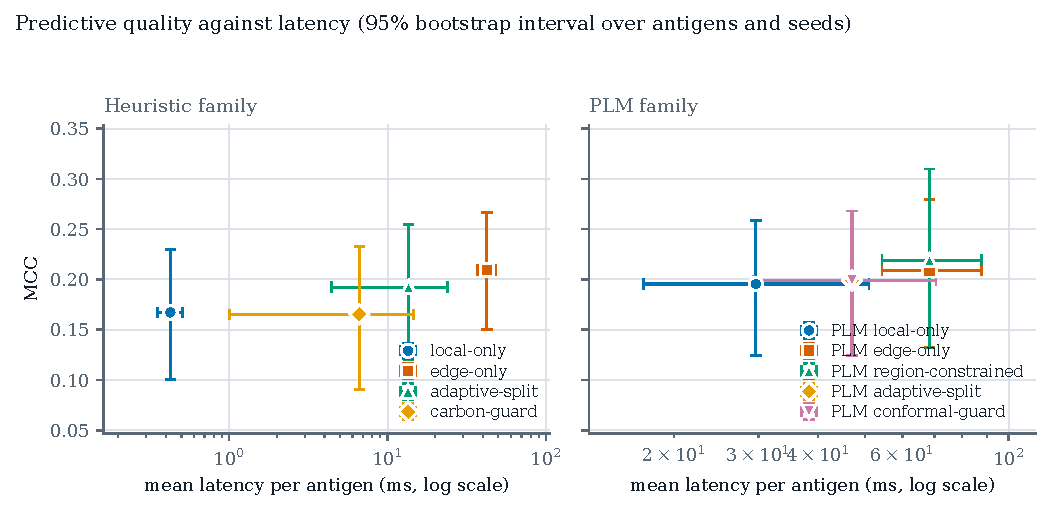
\includegraphics[width=\textwidth]{figures/fig_quality_latency.pdf}
\caption{Predictive quality against mean per-antigen latency on the BP3C50ID
external split, by policy family. Points are means over \NumSeeds{} seeds; bars
are 95\% bootstrap intervals on both axes. In the PLM panel the adaptive-split
and conformal-guard markers coincide exactly, because the conformal criterion
never altered a routing decision on this split.}
\label{fig:quality-latency}
\end{figure*}

\begin{figure*}[t]
\centering
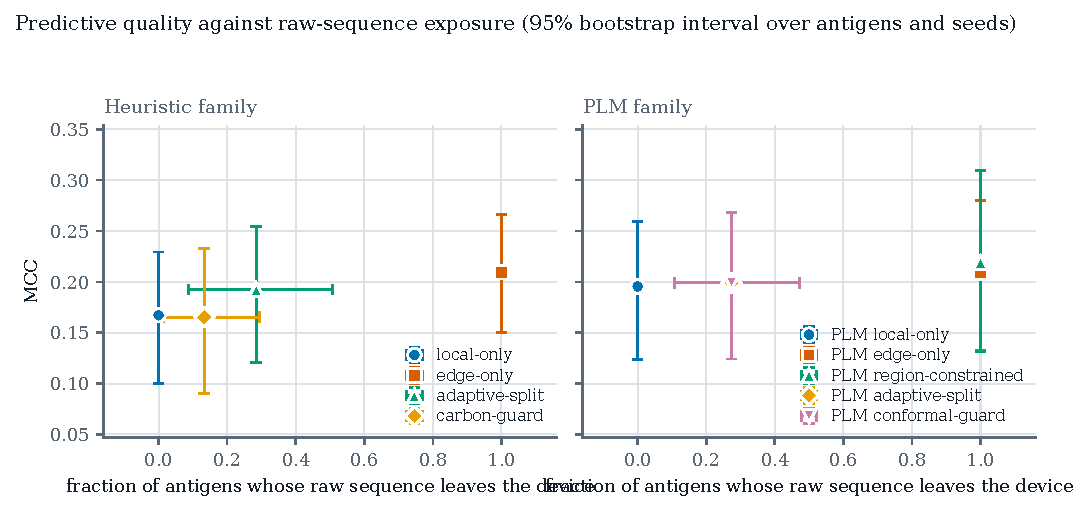
\includegraphics[width=\textwidth]{figures/fig_quality_datamovement.pdf}
\caption{Predictive quality against the fraction of antigens whose raw sequence
is transmitted. Policies at zero on the horizontal axis never transmit;
edge-only transmits every antigen. Adaptive-split occupies the interior of this
trade-off, which always-local and always-remote execution cannot.}
\label{fig:quality-data}
\end{figure*}

Table~\ref{tab:policy-summary} reports every policy on the BP3C50ID external
split across \NumSeeds{} seeds, and Table~\ref{tab:paired} gives the paired
comparisons that the claims below rest on.

Those five comparisons were fixed before the resampling was run: each contrasts
a routing policy with the always-local or always-remote baseline it is meant to
improve on, within its own predictor family. The resampling itself produces
intervals for all \PolicyPairsComputed{} orderable pairs of policies on each
metric, or \QualityIntervalsComputed{} intervals on the four quality metrics
together. We mark intervals that exclude zero in Table~\ref{tab:paired} as a
reading aid for those five rows, and no multiplicity correction is applied. A
reader should not treat the marks as a family-wise claim: across
\QualityIntervalsComputed{} intervals a handful would fall outside zero under
a global null, and several of the marked endpoints sit close enough to zero
that the Monte Carlo error of a \AntigenBootstrapRepeats{}-resample bootstrap
could move them. We draw no conclusion from any single mark, and the
conclusions below rest on the size and direction of the differences rather
than on which intervals happen to exclude zero.

Two points about those intervals before the results. They are two-way
bootstrap intervals over antigens and seeds
(\AntigenBootstrapRepeats{} resamples), not intervals over seeds alone. The
distinction is not cosmetic: the test split holds the same
\AntigenCount{} antigens in every seed, so a seed-only interval measures
how much a number moves when the harness is re-run and says nothing about how
it would move on different antigens. On this data seed-only intervals
are roughly an order of magnitude narrower: local-only MCC is
\ALocalOnlyMcc{} [\ALocalOnlyMccLo{}, \ALocalOnlyMccHi{}] under antigen
resampling against a seed-only width of a hundredth. For two of the
policies the seed-only ROC-AUC interval has width zero, because the underlying
predictor is deterministic and only the validation split moves. Every interval
below is the antigen-level one. We report it this way because the claims are
claims about antigens.

The first result is that the latency and disclosure benefits of routing are
large and survive this resampling, while the quality questions do not resolve
at this sample size. Figure~\ref{fig:quality-latency} plots predictive quality
against mean
per-antigen latency for each policy family.

Against always-remote execution, adaptive-split cuts mean latency by
\(\ADAsVsEoLatency{}\,\)ms [\ADAsVsEoLatencyLo{}, \ADAsVsEoLatencyHi{}] and
reduces the fraction of antigens whose raw sequence is transmitted by
\ADAsVsEoRawShare{} [\ADAsVsEoRawShareLo{}, \ADAsVsEoRawShareHi{}]
(Figure~\ref{fig:quality-data} shows quality against that fraction). Neither
difference could have come out positive: a policy that routes some antigens
cannot be slower than one that routes all of them, and cannot transmit more
sequences. These intervals therefore say how large the gain is on other
antigens, not whether there is one. On quality it differs by
\(\Delta\)MCC \ADAsVsEoMcc{} [\ADAsVsEoMccLo{}, \ADAsVsEoMccHi{}],
\(\Delta\)ROC-AUC \ADAsVsEoAuc{} [\ADAsVsEoAucLo{}, \ADAsVsEoAucHi{}],
\(\Delta\)AP \ADAsVsEoAp{} [\ADAsVsEoApLo{}, \ADAsVsEoApHi{}] and \(\Delta\)F1
\ADAsVsEoFOne{} [\ADAsVsEoFOneLo{}, \ADAsVsEoFOneHi{}]. All four contain zero.

We want to be careful about what that does and does not license. It is not a
demonstration of equivalence. With \AntigenCount{} antigens the interval on
\(\Delta\)MCC spans roughly \(\pm 0.05\), so a quality loss large enough to
matter in practice would not be detected here. The defensible statement is that
routing's quality cost relative to always-remote execution is not resolved at
this sample size, while its latency and disclosure benefits are.

The comparison against always-local execution tells the same story from the
other side. \(\Delta\)MCC is \ADAsVsLoMcc{}
[\ADAsVsLoMccLo{}, \ADAsVsLoMccHi{}], \(\Delta\)ROC-AUC \ADAsVsLoAuc{}
[\ADAsVsLoAucLo{}, \ADAsVsLoAucHi{}] and \(\Delta\)AP \ADAsVsLoAp{}
[\ADAsVsLoApLo{}, \ADAsVsLoApHi{}], all containing zero, while
\(\Delta\)F1 is \ADAsVsLoFOne{} [\ADAsVsLoFOneLo{}, \ADAsVsLoFOneHi{}], which
does not. One metric of four separates them. Under seed-only resampling the
same comparison appears decisive on every metric, with \(\Delta\)MCC
\DAsVsLoMcc{} [\DAsVsLoMccLo{}, \DAsVsLoMccHi{}] and a sign test over seeds at
\(p=\SAsVsLoMccP{}\). That sign test is a statement about ten re-runs on fifteen
fixed antigens, and we no longer rest anything on it.

Two comparisons do survive. The carbon-guard policy is worse than adaptive-split
on three of four metrics (\(\Delta\)MCC \ADCgVsAsMcc{}
[\ADCgVsAsMccLo{}, \ADCgVsAsMccHi{}]), so its latency and carbon savings are
bought with quality. Within the PLM family, always-remote execution beats
always-local on ROC-AUC and average precision. PLM routing gives part of
that back (\(\Delta\)ROC-AUC \ADPasVsPeoAuc{}
[\ADPasVsPeoAucLo{}, \ADPasVsPeoAucHi{}] against PLM always-remote): in the
family where the remote model is genuinely stronger, routing's quality cost is
detectable even here.

Table~\ref{tab:scenarios} reports the robustness axes the harness provides. The
informative row is the one where the remote tier is unavailable: every
adaptive-versus-local difference is then exactly zero, because routing degrades
to local-only behaviour rather than failing. The grid-intensity axes move
nothing that matters, and the parameter the carbon results are most sensitive
to --- the embodied amortisation constant --- is not among the available axes
(Section~\ref{sec:limitations}).


\begin{table}[t]
\centering
\caption{Sensitivity of the adaptive-split comparisons to the scenario axes available in the harness. Values are mean $\Delta$MCC over seeds. The grid-intensity axes do not touch predictive quality by construction and are included to show which axes were varied; the remote-tier-unavailable row is the informative one, where routing degrades exactly to always-local behaviour. The dominant carbon parameter, the embodied amortisation constant, is not among the available axes.}
\label{tab:scenarios}
\small
\begin{tabular}{lrr}
\toprule
Scenario & $\Delta$MCC vs local-only & $\Delta$MCC vs edge-only \\
\midrule
baseline & +0.034 & -0.010 \\
remote tier unavailable & +0.000 & +0.000 \\
network $+\SI{50}{\milli\second}$ & +0.034 & -0.010 \\
network $+\SI{5}{\milli\second}$ & +0.034 & -0.010 \\
grid intensity $\times 1.5$ & +0.034 & -0.010 \\
grid intensity $\times 0.5$ & +0.034 & -0.010 \\
\bottomrule
\end{tabular}
\end{table}


\begin{figure*}[t]
\centering
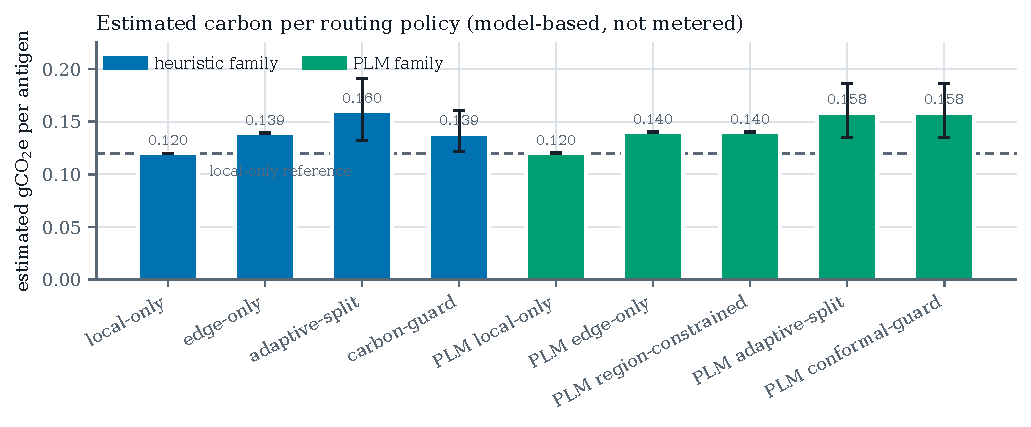
\includegraphics[width=\textwidth]{figures/fig_carbon.pdf}
\caption{Modelled carbon per antigen by policy, with 95\% intervals. These are
outputs of the energy model described in Section~\ref{sec:cost-accounting},
computed from fixed device power, an amortised embodied term and measured
latency; they are not metered measurements. Uncertainty-triggered routing is
the most carbon-intensive policy here because a routed antigen is charged two
device-requests; the ordering is specific to this checkpoint pair and reverses
for a larger remote tier, as the text below sets out.}
\label{fig:carbon}
\end{figure*}

\begin{table}[t]
\centering
\caption{Provenance of each reported cost quantity. Only latency is measured; the energy and carbon figures are derived from fixed device power and a grid-intensity constant, and are therefore model outputs rather than measurements.}
\label{tab:provenance}
\small
\begin{tabular}{ll}
\toprule
Quantity & Provenance \\
\midrule
Latency & timed benchmark execution \\
Energy & estimated from fixed power and latency \\
Operational carbon & estimated from energy and grid intensity \\
Embodied carbon & amortized estimate from device metadata \\
\bottomrule
\end{tabular}
\end{table}


The second result runs against the expectation that motivated the policy.
Figure~\ref{fig:carbon} shows modelled carbon per antigen for every policy.
Adaptive-split is the \emph{highest} of the nine at
\AdaptiveSplitCarbon{}~gCO\textsubscript{2}e
[\AdaptiveSplitCarbonLo{}, \AdaptiveSplitCarbonHi{}], above both edge-only
(\EdgeOnlyCarbon{}) and local-only (\LocalOnlyCarbon{}). The paired difference
against local-only is \DAsVsLoCarbon{} [\DAsVsLoCarbonLo{}, \DAsVsLoCarbonHi{}]
and against edge-only \DAsVsEoCarbon{} [\DAsVsEoCarbonLo{}, \DAsVsEoCarbonHi{}],
both intervals excluding zero.

This ordering is not an empirical discovery. Because a routed antigen incurs
the local pass that
decided to route it and then the remote pass, the modelled carbon of the
routing policy is determined by the two single-tier costs and the
routed fraction $r$:
\begin{equation}
C_{\text{adaptive}} \;=\; C_{\text{local}} \;+\; r\,C_{\text{edge}}.
\label{eq:carbon-identity}
\end{equation}
Equation~\ref{eq:carbon-identity} reproduces the measured aggregate to within
\CarbonIdentityError{}\% (predicted \CarbonPredictedAdaptive{} against measured
\AdaptiveSplitCarbon{}). Rearranging, routing costs more than always-remote
execution exactly when
\begin{equation}
r \;>\; 1 - \frac{C_{\text{local}}}{C_{\text{edge}}},
\label{eq:carbon-threshold}
\end{equation}
which for this device pair is \CarbonBreakEvenRate{}. The policy routes
\AdaptiveSplitRouteRate{} of antigens, roughly twice that threshold, so it
lands on the unfavourable side.

Stated this way the result transfers. Equation~\ref{eq:carbon-threshold} says
routing saves modelled carbon only where the local tier is cheap relative to
the remote tier \emph{and} the routed fraction stays below
$1 - C_{\text{local}}/C_{\text{edge}}$. That is the offloading energy threshold
of \citet{kumar2010cloud} written for this cost model, and our system falls on the
wrong side of it because per-residue screening on short
sequences makes the gating pass a large fraction of the work it gates. The
same inversion has been reported for draft-and-verify decoding cascades
\citep{dutta2026speculative}. What the measurements contribute is the location
of the threshold for this task, not the existence of one.

That location, however, is a property of the checkpoint pair rather than of
the task, and it does not survive a larger remote tier. In the recorded cost
model the embodied charge dominates: operational cost is
\ScaleOperationalShareEdge{}\% of the remote total, and the embodied term is
levied per request and does not grow with model size. Scaling the remote model
therefore grows a term that starts small, and
Equation~\ref{eq:carbon-threshold} moves only once it becomes comparable to
the embodied charge. Taking operational cost to scale with parameter count at
fixed sequence length (Figure~\ref{fig:selection-bias}, right), the break-even
fraction rises from
\ScaleBreakEvenMeasured{} at the \(8\)M remote tier measured here to
\ScaleSmallBreakEven{} at \(35\)M, \ScaleMidBreakEven{} at \(150\)M and
\ScaleLargeBreakEven{} at \(650\)M. Solving for the crossing exactly, the
ordering reverses once the remote call costs
\ScaleCrossoverFactor{}\(\times\) the one measured here, which is a remote
model of roughly \ScaleCrossoverParams{}M parameters at this local scale.

This matters for the claim rather than for the arithmetic. BepiPred-3.0, the
reference predictor a laboratory would actually call remotely, is built on
ESM-2 650M --- five times past that crossing. Against a remote tier of that
size the policy's routed fraction of \AdaptiveSplitRouteRate{} sits well below
the break-even, and routing becomes the \emph{less} carbon-intensive choice,
not the more. We therefore state the carbon result conditionally: routing is
the most carbon-intensive policy of those compared \emph{for the checkpoint
pair measured here}, and the finding that transfers is
Equation~\ref{eq:carbon-threshold} together with the observation that a
gate is only worth its carbon when what it gates is substantially more
expensive than the gate. Our own pairing, an \(8\)M local model against an
\(8\)M remote one, is close to the worst case for that condition. The
sensitivity is modelled on the recorded constants, not metered, like the
carbon figures it extends.

The carbon-guard policy, which exists precisely to suppress unprofitable
routing, does reduce carbon to \CarbonGuardCarbon{} --- essentially
edge-only's figure --- and cuts latency furthest, to
\(\CarbonGuardLatency{}\,\)ms. It pays for this in quality: against
adaptive-split its \(\Delta\)MCC is \DCgVsAsMcc{}
[\DCgVsAsMccLo{}, \DCgVsAsMccHi{}], an interval that excludes zero, and its MCC
of \CarbonGuardMcc{} is statistically indistinguishable from doing no routing at
all. On this evaluation the carbon guard does not find a useful middle point; it
mostly turns routing off.

Within the PLM family the pattern is similar but compressed, and one component
turns out to do nothing. The conformal-guard policy produces per-seed metrics
identical to PLM adaptive-split on every metric we record, to the precision
stored in the artifacts: the conformal criterion never changed a routing
decision on this split. We report it as a null component rather than omitting
it. The region-constrained post-processor, by contrast, is the one PLM addition
that helps, improving on PLM local-only by \(\Delta\)MCC \DPreVsPloMcc{}
[\DPreVsPloMccLo{}, \DPreVsPloMccHi{}] at no latency cost relative to PLM
edge-only.

\subsection{Reproducing the previously reported fusion advantage}
\label{sec:replication}

Before re-estimating the fusion effect we checked that any change could be
attributed to the protocol rather than to our reimplementation. The
original selection rule blends raw scores, scans the weight grid on the
evaluation split, and sets the threshold to preserve the reference predictor's
positive-call count on that split. Run through the loaders and metric code used
throughout this paper, it reproduces the earlier analysis. All
\TunedBpThreeReplicationRows{} entries of its stored weight-sensitivity grid
agree to within \TunedBpThreeReplicationMaxDiff{}, inside the
\TunedBpThreeReplicationTolerance{} tolerance the check applies and consistent
with the precision at which that grid was rounded. The procedure independently
selects the same optimum, \(w=\TunedBpThreeWeight{}\), and the same
positive-call count of \TunedBpThreePositiveCalls{}. This comparison is
executed by the replication script and its outcome recorded in the artifact
(status: \TunedBpThreeReplicationStatus{}) rather than asserted here.
Differences between the two protocols below are therefore attributable to how
the configuration is chosen rather than to a difference in implementation.

\subsection{The fusion advantage does not survive nested selection}
\label{sec:fusion-results}


\begin{table*}[t]
\centering
\caption{The fusion effect under two selection protocols. The test-derived protocol chooses the mixing weight and the decision threshold on the same split it reports; the nested protocol chooses both inside the training folds of a leave-one-sequence-out loop. Intervals are 95\% bootstrap intervals over per-antigen differences.}
\label{tab:fusion}
\small
\setlength{\tabcolsep}{4pt}
\begin{tabular}{@{}llrrrr@{}}
\toprule
Split & Protocol & Weight & $\Delta$ROC-AUC & $\Delta$MCC & Antigens improved \\
\midrule
BP3C50ID external test & test-derived & 0.90 & +0.0018 & +0.0115 & -- \\
 & nested (LOSO) & 0.90 & -0.0005 & -0.0329 & 7/15 \\
 & & \tiny[0.55, 0.90] & \tiny[-0.0033, +0.0021] & \tiny[-0.0955, +0.0088] & \\
\addlinespace
IEDB bounded subset & test-derived & 0.95 & +0.0012 & +0.0012 & -- \\
 & nested (LOSO) & 0.95 & +0.0008 & +0.0014 & 25/47 \\
 & & \tiny[0.85, 0.95] & \tiny[-0.0010, +0.0027] & \tiny[-0.0037, +0.0066] & \\
\bottomrule
\end{tabular}
\end{table*}


\begin{figure*}[t]
\centering
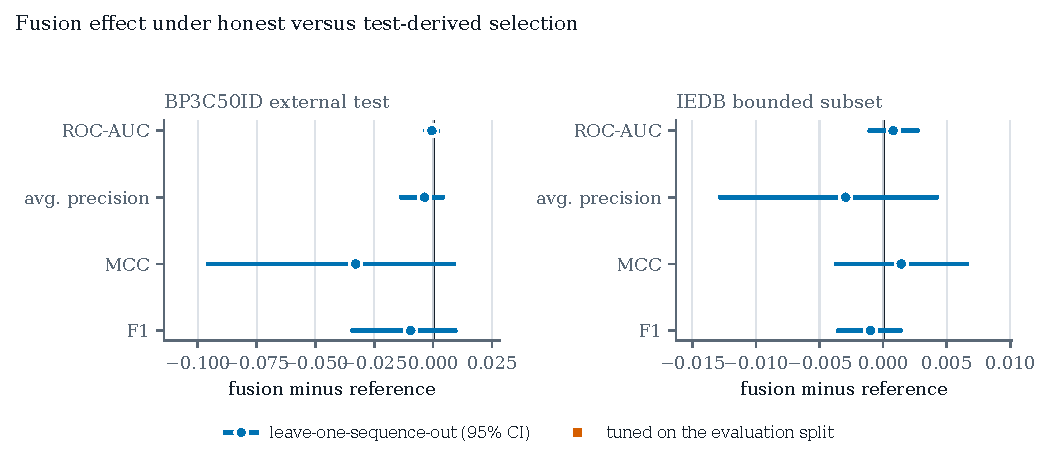
\includegraphics[width=\textwidth]{figures/fig_fusion_forest.pdf}
\caption{The fusion effect against the reference predictor under two selection
protocols. Blue intervals are mean per-antigen differences with 95\% bootstrap
intervals under leave-one-sequence-out nested selection; orange squares are the
corresponding estimates when the weight and threshold are chosen on the
evaluation split. On both datasets the nested interval contains zero while the
test-derived estimate sits above it.}
\label{fig:fusion-forest}
\end{figure*}

\begin{figure*}[t]
\centering
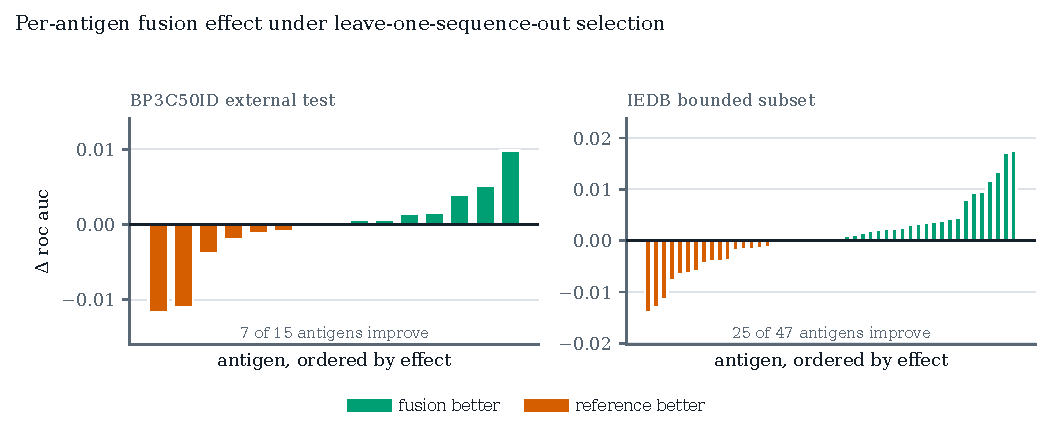
\includegraphics[width=\textwidth]{figures/fig_per_sequence.pdf}
\caption{Per-antigen change in ROC-AUC from fusion under nested selection,
ordered by effect. The dispersion, particularly on the IEDB subset, is much
larger than the mean effect in either direction.}
\label{fig:per-sequence}
\end{figure*}

Table~\ref{tab:fusion} and Figure~\ref{fig:fusion-forest} give both protocols on
both datasets.

On BP3C50ID, nested selection leaves a mean per-antigen difference against
BepiPred-3.0 of \NestedBpThreeDeltaAuc{} ROC-AUC
[\NestedBpThreeDeltaAucLo{}, \NestedBpThreeDeltaAucHi{}], with
\NestedBpThreeWinsAuc{} of \NestedBpThreeSequences{} antigens improving and a
Wilcoxon $p$ of \NestedBpThreePAuc{}. MCC behaves the same way
(\NestedBpThreeDeltaMcc{} [\NestedBpThreeDeltaMccLo{}, \NestedBpThreeDeltaMccHi{}],
$p=\NestedBpThreePMcc{}$).

The larger IEDB subset behaves the same way, with one important difference in
what it tests. We have no BepiPred-3.0 predictions for those antigens, so that
arm fuses the candidate with our own local-only predictor rather than with
BepiPred-3.0. It is a second instance of the same selection question, not a
replication of the same comparison, and we do not read it as independent
confirmation of the BepiPred-3.0 result. The mean per-antigen
difference in ROC-AUC is \NestedIedbDeltaAuc{}
[\NestedIedbDeltaAucLo{}, \NestedIedbDeltaAucHi{}], with
\NestedIedbWinsAuc{} of \NestedIedbSequences{} antigens improving
($p=\NestedIedbPAuc{}$), and MCC gives \NestedIedbDeltaMcc{}
[\NestedIedbDeltaMccLo{}, \NestedIedbDeltaMccHi{}]. Every interval on both
datasets contains zero. Both the Wilcoxon test and the sign test discard
antigens whose paired difference is exactly zero; on BP3C50ID this removes
\NestedBpThreeTiesAuc{} antigens for ROC-AUC and \NestedBpThreeTiesMcc{} for
MCC, and on the IEDB subset \NestedIedbTiesAuc{} and \NestedIedbTiesMcc{}, so
the effective sample size is smaller than the stated number of antigens by
that count.

We are careful about what these nulls support. An interval containing zero is
not evidence that the effect is zero, and at these sample sizes the paired
design cannot resolve effects of the size at issue. With the observed
per-antigen dispersion, the smallest difference BP3C50ID could detect with
80\% power at a two-sided 5\% level is \NestedBpThreeMdeMcc{} in MCC and
\NestedBpThreeMdeAuc{} in ROC-AUC; on the IEDB subset the corresponding
figures are \NestedIedbMdeMcc{} and \NestedIedbMdeAuc{}. The MCC effect the
test-derived protocol reports, \TunedBpThreeDeltaMcc{}, is far below what the
nested analysis could have detected. A non-significant nested result was close
to guaranteed, so it carries little evidential weight against that specific
effect.

What the design does identify is the behaviour of the estimator. Under the
test-derived protocol the same BP3C50ID data yield \TunedBpThreeDeltaMcc{} MCC
and \TunedBpThreeDeltaAuc{} ROC-AUC in favour of fusion; under nested
selection the same quantity on the same data is \NestedBpThreeDeltaMcc{} and
\NestedBpThreeDeltaAuc{}. The point estimate does not shrink towards zero, it
changes sign. That is a statement about how much the selection step moves the
estimate, which this comparison does identify, rather than a statement about
the underlying effect, which it does not. The defensible conclusion is that
the test-derived estimate is biased by at least the distance between the two,
not that fusion does not help.

Figure~\ref{fig:per-sequence} shows the per-antigen differences behind these
means. The dispersion is far larger than the mean in both directions. That is
what a null effect over a small number of antigens looks like, and it is the
reason we report the paired tests rather than a pooled number alone.

\subsection{How often the published literature selects this way}
\label{sec:survey}

The result above is a correction to our own unpublished analysis, which bounds
how much it matters. To ask whether the practice is confined to us, we
surveyed published B-cell epitope predictors that combine two or more models
--- score fusion, ensembles, stacking, consensus voting --- and asked of each
whether the combination parameter was chosen using the same data the headline
performance is reported on. The survey covers
\SurveyAssessed{} assessable papers and records, for every one, the verbatim
sentence the judgement rests on; it is released with the code.

We keep three categories apart. \SurveyLeakage{} papers are \emph{leakage
evident}: the text states that a mixing weight, a voting rule, an ensemble
composition or a reported configuration was chosen by inspecting performance
on the evaluation data. \SurveyClean{} are \emph{leakage-free evident}: a
validation split, the training set, or a rule fixed a priori.
\SurveyUnreported{} are \emph{unreported}: the paper does not say on which
data the parameter was chosen. We do not count the third group as leakage. It
is an observation about what the methods section contains, and its size is
itself the point --- a quarter of the sample does not let a reader check.
Among the \SurveyStatingBasis{} papers that do state a basis,
\SurveyLeakageShare{}\% selected on their own evaluation data.

These counts are not a prevalence estimate and we do not offer them as one.
The sample is open-access only, reachable by keyword, and skewed towards
recent and prominent work; paywalled methods papers are structurally absent.
With \SurveyAssessed{} papers each count carries a sampling error of one or
two. What the survey does establish is that the selection step we found in our
own work is present in the published literature, that it is not rare among
papers that disclose enough to tell, and that a substantial minority of papers
disclose too little for the question to be asked at all. The magnitude such a
step can reach is the subject of the next section.

\subsection{How large the selection step is, and what governs it}
\label{sec:bias-curve}

The sections above establish that the selection step moved our estimate and
that the practice occurs in print. Neither says how large an effect a reader
should expect it to produce. That is answerable from the same data by
resampling.

For a given antigen count and weight grid we draw a subset without
replacement, estimate the fused-minus-reference difference on it twice, and
record the gap. The first estimate scans the grid on the subset and keeps the
best row, which is the protocol a paper follows when it reports a tuned
combination parameter without holding anything out. The second applies
leave-one-sequence-out selection inside the same subset. Both estimators see
exactly the same antigens, so the gap is attributable to the selection rule
rather than to which data were drawn. We average over \BiasReplicates{} draws
per cell.

\begin{figure*}[t]
\centering
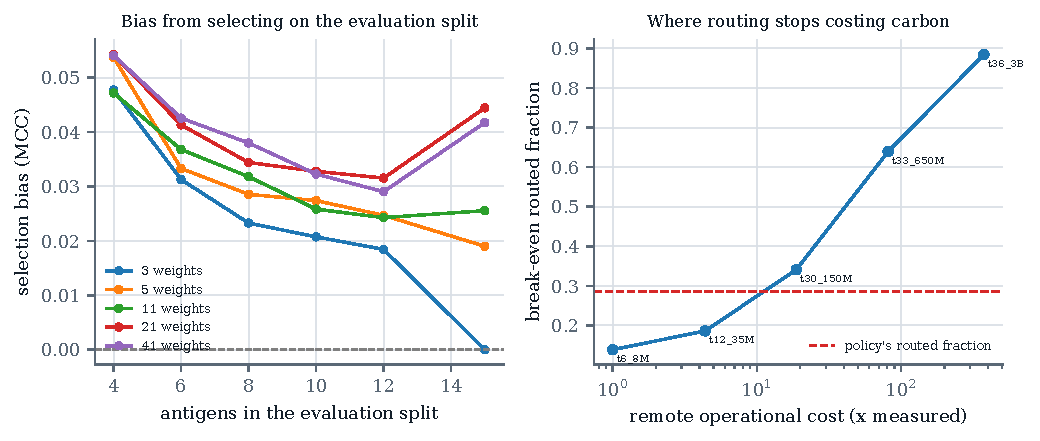
\includegraphics[width=\textwidth]{figures/fig_selection_bias.pdf}
\caption{Left: the mean gap between a weight chosen on the evaluation split
and one chosen by leave-one-sequence-out selection within it, over
\BiasReplicates{} draws per cell, by antigen count and weight-grid density.
Both estimators see the same antigens in every draw. The rightmost point of
each series is the full split, where only one subset exists; it is a single
deterministic run rather than a mean, which is why the coarsest grid reaches
exactly zero there, and it should not be read as part of the trend. Right:
the break-even routed fraction of
Equation~\ref{eq:carbon-threshold} as the remote tier is scaled, with the
policy's own routed fraction marked. The released ESM-2 checkpoints are
labelled; the ordering reverses between \(35\)M and \(150\)M. Both panels
are modelled from the recorded constants, not metered.}
\label{fig:selection-bias}
\end{figure*}

The bias is positive everywhere and large relative to the effects this
literature reports (Figure~\ref{fig:selection-bias}, left). On \BiasMetric{}
it runs from \BiasAtSmallestN{} at
\BiasSmallestN{} antigens to \BiasAtLargestN{} at \BiasLargestN{}. It grows
with the density of the grid: at \BiasGridRefN{} antigens a
\BiasCoarseGridPoints{}-point grid yields \BiasCoarseGridBias{} and a
\BiasFineGridPoints{}-point grid \BiasFineGridBias{}, which is what one would
expect if a finer scan simply offers more chances to fit the evaluation split.
At the grid densities ordinarily used --- weight steps of \(0.05\) are
common --- the test-derived estimate was the more favourable one in
\BiasPositiveShareLargestN{}\% of draws. The full-split cell reproduces the
headline of Section~\ref{sec:fusion-results} exactly, at
\BiasAtLargestN{}, which is the difference between the
\TunedBpThreeDeltaMcc{} that protocol reports and the
\NestedBpThreeDeltaMcc{} nested selection returns.

The comparison worth drawing is between that bias and the effects it is used
to support. Our own earlier analysis reported a gain of
\TunedBpThreeDeltaMcc{} \BiasMetric{}. The expected bias at that sample size
and grid density is several times larger. A tuned fusion result of that
magnitude, on a benchmark of this size, therefore carries no information about
whether fusion helps: it is within what the selection rule alone produces.
This is the sense in which the present work generalises beyond one corrected
analysis. The bias is not an accident of our predictors; it is a property of
scanning a grid on a small evaluation set, and its size can be estimated in
advance for any such design.

We are careful about the scope. These magnitudes are specific to these two
predictors, whose mean rank agreement across cells is \BiasAgreement{}; two
predictors that agree less would leave more room for a scan to exploit, and
two that agree more would leave less. What transfers is the construction and
the direction, not the numbers.

\subsection{Which predictor the procedure prefers}
\label{sec:weight-transfer}

\begin{figure*}[t]
\centering
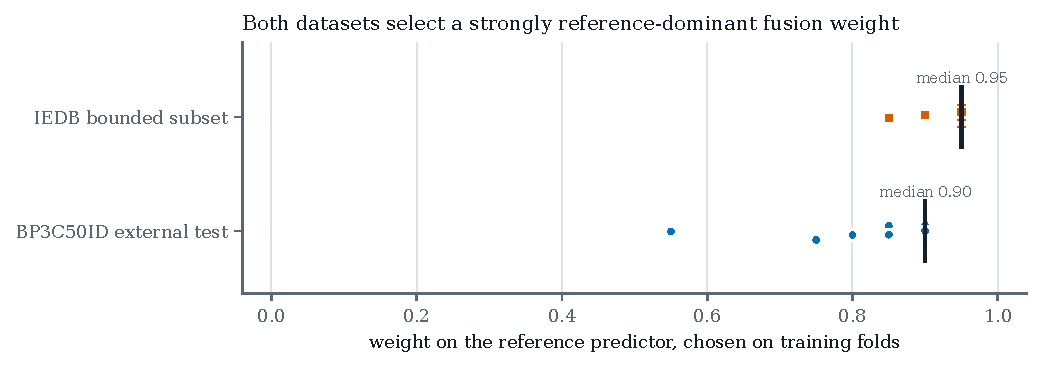
\includegraphics[width=\textwidth]{figures/fig_weight_stability.pdf}
\caption{The fusion weight selected in each training fold, by dataset, with
medians marked. Both datasets place almost all of the weight on the reference
predictor, which is the same conclusion the null effect reaches by a different
route.}
\label{fig:weight-stability}
\end{figure*}

Figure~\ref{fig:weight-stability} plots the weight chosen in each training fold.
On BP3C50ID the folds settle around a median of \NestedBpThreeWeightMedian{}
(range \NestedBpThreeWeightMin{} to \NestedBpThreeWeightMax{}); on the IEDB
subset the median is \NestedIedbWeightMedian{} (range \NestedIedbWeightMin{} to
\NestedIedbWeightMax{}). Both sit close to the upper end of the grid, meaning
the selection procedure chooses to give our predictor almost no influence over
the blended score.

The selected weights are an independent route to the same
conclusion. The nested evaluation says the blend cannot be distinguished from
the reference predictor. The selected weights say why: the
procedure, given a free choice, declines to use the second predictor. A fusion
whose fitted weight approaches one is not a combination of two models but the
stronger model with extra machinery attached.

\section{Discussion}
\label{sec:discussion}

\subsection{Routing is a disclosure and latency mechanism, not a green one}

The case for local--edge routing in a screening pipeline is sound, but it is a
different case from the one usually made, and narrower than we expected to be
able to make. On our evaluation the mechanism buys two things a laboratory can
verify directly, and both survive antigen-level resampling. Screening finishes
in roughly a third of the time always-remote execution takes. Most antigens are
never transmitted. The second gain is not obtainable by buying a faster remote
service.

What it does not buy, on evidence of this size, is a demonstrated quality
position. Against always-remote execution the quality difference is not
resolved; against always-local execution only one metric of four separates
them. We had originally read the same comparisons as decisive, on intervals
computed over seeds, and Section~\ref{sec:routing-results} explains why those
were the wrong intervals. A laboratory deciding whether to adopt routing should
therefore treat the latency and disclosure gains as established here and the
quality question as open. That is a less satisfying recommendation than the one
we set out to make. It is also a more defensible one.

What the mechanism does not buy is lower energy, and
Equation~\ref{eq:carbon-threshold} says precisely when it would. Offloading
saves energy only above a ratio of work offloaded to overhead incurred
\citep{kumar2010cloud}. Our contribution is to locate that boundary for this
task, at a routed fraction of \CarbonBreakEvenRate{}, and to observe that a
policy tuned for predictive quality routes about twice as often as that. The
green argument
would recover for longer antigens or a heavier remote tier, where the ratio
shifts. Practitioners can evaluate Equation~\ref{eq:carbon-threshold} for their
own pair rather than assuming either direction.

The practical recommendation, then, is to adopt routing when sequence disclosure
or turnaround is the binding constraint, and not to adopt it on environmental
grounds without measuring the ratio for the models actually in use.

\subsection{What the fusion result means, and what it does not}

Our result is that a convex blend of CARBON-BCE-R with BepiPred-3.0 shows no
advantage over BepiPred-3.0 alone, on either of two datasets, once the blend is
chosen without reference to the evaluation labels. The scope of that claim
matters.

It is not a claim that score fusion is useless in epitope prediction. It is a
claim about one pair of predictors on two splits. One member of that pair is
considerably weaker than the other, and the folds consistently chose to
down-weight the weaker member. A fusion of two comparably strong and genuinely
complementary predictors might well behave differently. Nothing here tests that.

It is also not a claim that the earlier result was dishonestly produced. The
protocol that generated it is easy to arrive at by accident, because a weight
sweep serves two different purposes that look the same on the page. Presented as
a sensitivity analysis, it answers "how fragile is this result to the weight?"
Used to pick the reported row, it answers "what is the best this combination can
look like?" The second question's answer is then reported as though it were the
first's. The diagnostic is procedural rather than statistical: ask whether the
configuration being reported was selected using the labels it is scored against.

What the result does establish is that in this corner of the literature the
difference between the two protocols is large enough to manufacture a positive
finding out of a null one, on data where the optimistic protocol produced a
plausible-looking effect with a bootstrap interval attached. Reporting an
interval does not protect against selection bias when the selection happened
before the interval was computed. Given how inexpensive the nested alternative
is --- one extra loop over
sequences, no new data, no new model --- we think it should be the default
whenever a combination parameter is tuned on a dataset of this size.

\subsection{Relation to prior work}

Our benchmark is built on the BP3C50ID split distributed with BepiPred-3.0
\citep{clifford2022bepipred}. The local predictor descends from the
feature-based and deep approaches surveyed by \citet{cia2023critical} and
exemplified in this journal by \citet{attique2023deepbce}. We do not advance the
state of the art in predictive accuracy and do not claim to. Standalone
CARBON-BCE-R remains below BepiPred-3.0 on BP3C50ID, and structure-aware methods
such as DiscoTope-3.0 \citep{hoie2024discotope} occupy ground our sequence-only
setting does not reach.

Our evaluation is small beside purpose-built benchmarks for this area such as
AsEP \citep{liu2024asep}, and we call it a measurement harness rather than a
benchmark for that reason. Within the scope of inference routing, however, we
are not aware of prior work that routes between a local and a remote
conformational epitope predictor and measures the consequences. Federated
approaches to protein modelling address a different problem. They distribute
training rather than place inference.

The systems contribution sits alongside the split-computing literature
\citep{matsubara2022split}, from which the routing mechanism is borrowed rather
than invented. What we add is the measurement of that mechanism against the
objectives a wet-lab screening workflow actually has. That includes the
counting measure of raw-sequence disclosure, which accuracy-oriented
formulations do not express, and the observation that the energy argument
inverts at this scale.

The methodological contribution is an instance of the problem
\citet{kapoor2023leakage} document across applied machine-learning fields,
reported from the inside: we are correcting our own earlier result rather than
auditing someone else's. We think instances of this kind are useful precisely
because the published record contains few of them.

\section{Limitations}
\label{sec:limitations}

Several constraints bound what can be concluded from this study.

\paragraph{Carbon is modelled, never metered.} Every energy and carbon figure in
this paper is computed from a fixed device power constant, a measured latency
and a grid-intensity constant (Section~\ref{sec:cost-accounting},
Table~\ref{tab:provenance}). No wall-power measurement was taken at any point.
The carbon comparisons between policies are therefore comparisons of modelled
quantities that are proportional to measured latency; they support statements
about which policy does more work, and they do not support any statement about
emissions of a deployed system. A metered replication on instrumented hardware
is the obvious next step and is not something this study attempted.


\paragraph{The carbon figures rest on two utilisation constants.} The energy
model reproduces, but only once the utilisation fractions are
supplied by hand. Across all \CarbonSequencesChecked{} antigens of the second
dataset, recomputing each per-antigen total from the recorded device
configuration, the measured latencies and the utilisation fractions of
Section~\ref{sec:cost-accounting} matches the stored values to within
\CarbonReconstructionError{}~gCO\textsubscript{2}e. The fractions are not in
the recorded configuration, so the stored totals cannot be rebuilt from that
configuration alone, and the released decomposition artifact says so. The
fractions themselves,
however, are literals in the benchmark code rather than entries in any
configuration file, and they dominate the result: the embodied term is almost
the whole of each per-request total.

That matters for how far the carbon conclusion travels. Of
\CarbonFractionSettingsTested{} alternative settings we evaluated, the ordering
survives in all but \CarbonFractionSettingsFlipping{}. A device pair with the
local tier at \CarbonFlipLocalFraction{} utilisation and the remote tier at
\CarbonFlipEdgeFraction{} would put the break-even routed fraction at
\CarbonFlipBreakEven{}, above the rate our policy actually routes at. Routing
would then be the greener option. Our finding therefore holds for the hardware
pair modelled here and for most reasonable variations on it. It remains a
statement about a cost model whose dominant parameters deserve to be measured
rather than assumed. A metered replication remains the right next
step.

\paragraph{The remote tier is co-located, not remote.} The latency figures
attribute a transport cost to routed antigens, but the benchmark executes both
tiers on one machine, and the two-node transport evidence in the artifact is an
HTTP probe, not a deployed remote model server. Real deployments would
add network variance, queueing and failure modes that
this harness does not model. For latency and for transmitted volume these
would, if anything, favour routing, not count against it, since
always-remote execution pays the network on every antigen and routing pays it
on roughly a quarter. What a real deployment would add against routing is of a
different kind: a dependency on the remote tier for exactly the antigens the
local model found hardest, and the failure and retry behaviour that comes with
it. We measure none of that.


\paragraph{The primary benchmark is small, and that bounds nearly everything.}
BP3C50ID's external split has \BepipredNumAntigens{} antigens. Resampling on
\BepipredNumAntigens{} units gives intervals wide enough that most quality
comparisons in this paper are not resolved, and every such comparison should be
read as "no effect detectable at this sample size" rather than as "no effect".
This applies to the routing results as much as to the fusion analysis: the
interval on the adaptive-split versus always-remote MCC difference spans roughly
$\pm 0.05$, which would not exclude a quality loss a practitioner would care
about. For the fusion analysis the IEDB subset at \NestedIedbSequences{}
antigens carries more weight on ROC-AUC and average precision, where it has no
tied folds. On the threshold-dependent metrics its informative-fold count is
closer to BP3C50ID's and we do not claim it is better powered there.

\paragraph{The language-model tier is the smallest available checkpoint.} The
PLM results use \texttt{esm2\_t6\_8M\_UR50D}, chosen for the hardware at hand.
Conclusions about the PLM family are conclusions about an 8M-parameter frozen
encoder and should not be read as characterising what language-model features
can contribute to this task.

\paragraph{One routing signal, one validation design.} Routing decisions come
from mean per-residue local uncertainty, selected on a single grouped validation
split per seed. Repeated grouped resampling of the validation split would give a
better picture of how stable the selected thresholds are; we vary the seed,
which moves the split, but we do not separate the two sources of variation.

\paragraph{The IEDB subset's sampling rule is not recorded.} Its source and
identity filter are established (Section~\ref{sec:datasets}), but how the
\IedbSubsetTest{} test and \IedbSubsetTrain{} training antigens were drawn from
the \IedbSourceSequences{} available is not captured in any script we could
find. The selection is therefore reproducible in its inputs but not in its
sampling. We state this rather than reconstruct a rule after the fact, since a
plausible-looking rule invented now would be indistinguishable in the write-up
from one that was actually followed, which is the failure this paper is about.
What we can do is pin down the set: the released manifest lists every test
antigen by accession, so the evaluation subset is identified exactly even
though the draw that produced it is not. The consequence for the reader is
that the IEDB arm should be treated as a second dataset of opportunity rather
than as a designed replication, and we do not rest the paper's conclusions on
it.

\section*{Declarations}

\paragraph{Data and code availability.} The benchmark harness, the analysis
modules that produce every table and figure in this paper, and the raw
per-seed result artifacts are available at
\url{https://github.com/Anandharajan/edgeconbce}. A single command
(\texttt{regenerate.sh}) rebuilds the generated-number file, all tables, all
figures and this manuscript from the stored results. The repository is
archived on Zenodo at acceptance and the DOI will replace this URL in the
published version.

The BP3C50ID training and external test splits, and the
\texttt{\IedbSourceFile{}} collection from which the second evaluation set is
drawn, are redistributed by the Technical University of Denmark alongside
BepiPred-3.0. We do not republish them, and the repository contains no antigen
sequences from either source. The BepiPred-3.0 predictions used as the
reference were obtained from the official service.

The rule by which the \IedbSubsetTest{} test and \IedbSubsetTrain{} training
antigens were drawn from that collection was not recorded when the subset was
made, and we have not been able to recover it. We therefore release the
identity of the evaluation subset instead
(\texttt{data/iedb\_subset\_manifest.csv}), which lists every test antigen by
accession, so that the set itself can be reconstructed from the source
collection even though the draw cannot be repeated. The
\IedbSubsetTrain{} training antigens are counted in the released artifacts but
not identified, and we do not reconstruct them after the fact.

\paragraph{Ethics.} This study uses only published protein sequence data. No
human participants, human tissue, animal subjects or personally identifying
information were involved, and no ethics approval was therefore required.

\paragraph{Funding.} This research did not receive any specific grant from
funding agencies in the public, commercial, or not-for-profit sectors.

\paragraph{Competing interests.} The author declares that he has no known
competing financial interests or personal relationships that could have
appeared to influence the work reported in this paper.

\paragraph{Declaration of generative AI in the writing process.} During the
preparation of this work the author used generative AI tools to assist with
the work. The author reviewed and edited all content, verified every result
reported here, and takes full responsibility for the content of the published
article.

\paragraph{CRediT author statement.} \textbf{Anandharajan TRV:}
Conceptualization, Methodology, Software, Validation, Formal analysis,
Investigation, Data curation, Writing --- original draft, Writing --- review
and editing, Visualization, Supervision, Project administration.


\bibliographystyle{plainnat}
\bibliography{references}

\end{document}
